\documentclass[a4paper]{article}
\usepackage[utf8]{inputenc}
\usepackage[english, russian]{babel}
\usepackage{indentfirst}
\usepackage{amsmath,amsfonts,amssymb,amsthm,mathtools}
\usepackage{svg}
\usepackage{graphicx}
\usepackage{prftree}
\usepackage{multicol}
\usepackage[14pt]{extsizes}
\newtheorem{theorem}{Теорема}
\newtheorem*{theorem*}{Теорема}
\newtheorem{lemma}{Лемма}
\newtheorem*{lemma*}{Лемма}
\theoremstyle{definition}
\newtheorem{definition}{Определение}
\newtheorem*{definition*}{Определение}
\newtheorem*{name}{Обозначение}
\newtheorem*{exmp}{Пример}
\newtheorem*{paradoks}{Парадокс}
\newtheorem*{hypo}{Гипотеза}
\newtheorem{proposition}{Предложение}
\newtheorem*{proposition*}{Предложение}
\newtheorem*{comment*}{Замечание}
\newtheorem{comment}{Замечание}
\newtheorem*{upr}{Упражнение}
\newtheorem{upr*}{Упражнение}
\newtheorem{consequence}{Следствие}
\newtheorem*{consequence*}{Следствие}
\title{ Коллоквиум №1 (20.11.2019) }
\author{GROUPS №19137,№19144}
\date{2019\\}
\begin{document}
\maketitle
\begin{enumerate}
 \item Множество: способы задания, операции над множествами
       \\ Не существует явного определения множества.
       \\ Пусть A некоторое мн-во, тогда существует 3 способа задания мн-ва
       \begin{enumerate}
        \item A = \{1,2,3,4,5\} - явное задание эл-тов мн-ва \\
        \item Пусть $\Phi(x)$- некоторое условие, тогда \\A = $\{x \ | \ \Phi(x) \}$ - Задание множествами с помощью некоторого условия $\Phi(x)$
        \item С помощью рекуретного соотношения.\\
              Пример: $a_n$ - числа Фибоначчи, тогда \\
              $a_1=a_2=1$, $a_n = a_{n-1}+a_{n-2}$
       \end{enumerate}
       Пусть A, B- некоторые множества \\
       \begin{name}[Подмножетсво]
        A - подмножетсво B, если\\
        \mbox{$A \subseteq B = \{x \ | x\in{A} \Rightarrow x\in{B} \}$}
       \end{name}
       \begin{name}[Собстевенное подмножетсво]
        A - собстевенное подмножетсво B, если
        \mbox{$A \subset B$, если $A \subseteq B$ и $A\ne{B} $}
       \end{name}
       \begin{name}[Пустое множество]
        $\emptyset$ - множество, не содержащее эл-тов ("Пустое множество")
       \end{name}
       \begin{name}[Множество всех подмножетсв множества A]
        \mbox{}\\
        \mbox{$P(A) = \{ \ C\ |\ C \subseteq{A} \ \} $}
       \end{name}
       \begin{name}[Универсум]
        Универсум (условное множество все множеств) $U$
       \end{name}
       Операции над множествами:
       \begin{itemize}
        \item Объединение множеств:
              \\ $A\cup{B} = \{ x \ | \ x \in{A} \lor x\in{B}\}$
        \item Пересечение множеств:
              \\ $A\cap{B} = \{ x \ | \ x \in{A} \land x\in{B}\}$
        \item Разность множеств:
              \\ $A \ \backslash\  B = \{x\ | \ x\in{A} \land x\notin{B} \}$
        \item Дополнение множества:
              \\ $\neg{A} = \{\ x\ |\ x \in{\ U} \land{x \notin{A}}\} $
        \item Симметрическая разность множеств:
              \\ $A \ \Delta \ B = (A \  \backslash \ B) \cup{(B \ \backslash{\ A})} = (A\ \cup{\ B })\ \backslash \ (B\ \cap{\ A } ) $
       \end{itemize}
       Пусть S - семейство множеств:
       \begin{itemize}
        \item Объединение семейства множеств\\
              $\bigcup{S} = \{\ x\ |\ \exists{A_i} \in{\ S \ }:x\ \in{\ A_i \ }\}$
        \item Пересечение семейства множеств\\
              $\bigcap{S} = \{\ x\ |\ \forall{A_i} \in{\ S\ }: x\ \in{\ A_i \ } \}$
       \end{itemize}
 \item Упорядоченный набор (кортеж), предложение о равенстве n-ок, декартово произведение, декартова степень.
       \begin{definition*}[Упорядоченный набор (кортеж)]
        Упорядоченный набор (кортеж) длины n определяется по индукции
        \begin{math}\\
         <> = \emptyset\\
         <a> = a\\
         <a,b> = \{\{a\},\{a,b\}\}
         \\
         ...
         \\
         <a_1, a_2, ...,a_{n-1} ,a_n> = <<a_1, a_2, ...,a_{n-1})>, a_n>
        \end{math}
       \end{definition*}
       \begin{definition*}[пара]
        Набор $<a,b>$ длины 2 называют \textit{парой}
       \end{definition*}
       \begin{proposition*}[о равенстве n-ок]
        Если \\ \mbox{$<a_1,...,a_n> = <b_1, ..., b_n> \Leftrightarrow a_1 = b_1, ..., a_n = b_n$}
       \end{proposition*}
       \begin{proof}
        для $n=1$ очевидно в обе стороны. Докажем для $n = 2$: \\
        $<a_1, a_2> = <b_1, b_2> \Leftrightarrow \{\{a_1\},\{ a_1, a_2\} \} = \{\{b_1\},\{ b_1, b_2\}\}$
        \\ Пусть $a_1 = a_2 \Rightarrow \left[
         \begin{gathered}
          \{a_1\} = \{b_1, b_2\}\hfill \\
          \{a_1, a_2\} = \{b_1, b_2\}\hfill \\
         \end{gathered}
         \right. \Rightarrow a_1=a_2 = b_1 = b_2 $
        \\ для $b_1 = b_2$ аналогично.\\ Расмотрим $a_1 \ne a_2, b_1 \ne b_2$\\
        $\Rightarrow \left[ \begin{gathered}
          \{a_1\} = \{b_1\}\hfill \\
          \{a_1\} = \{b_1, b_2\}\hfill \\
         \end{gathered}
         \right. \xRightarrow[]{\text{Так как}\ b_1 \ne b_2} \{a_1\} = \{b_1\} \Rightarrow a_1 = b_1$\\
        \\По аналогии для $\{a_1, a_2\} = \{b_1, b_2\}$\\
        Т.к справледливо для $n=2$, а определение n-ок индуктивно следовательно верно для n
       \end{proof}
       \begin{definition*}[Декартово произведение]
        Пусть даны множества $A_1,...,A_n$, тогда их декартовым произведением называют
        \newline\mbox{$A_1 \times A_2 \times ... \times A_n = \{<a_1,...,a_n>|\  \forall{i}\in{\{1,...,n\}}\ a_i\in{A_i} \}$}
       \end{definition*}
       \begin{definition*}[Декартова степень]
        В случае, если \mbox{$A_1=A_2=...=A_n$}, тогда $A_1 \times A_2 \times ... \times A_n$ называют декартовой степенью и обозначают, как $A^n=A_1 \times A_2 \times ... \times A_n$
       \end{definition*}
       \newpage
 \item Бинарные отношения, обратное отношение, произведение отношений, лемма о бинарных отношениях.
       \begin{definition*}Бинарным отношением между элементами множеств A и B называется произвольное подмножество\\
        $C \subseteq{A \times B}$
       \end{definition*}
       \begin{definition*}Обратным бинарным отношением называется \\
        $R^{-1} = \{<y;x> |\ <x;y> \in{R}\}$
       \end{definition*}
       \begin{definition*}Произведением бинарных отношений называется \\
        $R_{1}\times R_{2} = \{<x;z>          |\exists y |\ <x;y> \in R_{1}   \land <y;z> \in R_{2}\}$
       \end{definition*}
       \begin{lemma*}[Лемма о бинарных отношениях]
        Для любых бинарных отношений $R_{1},R_{2},R_{3} $:
        \begin{enumerate}
         \item     $R_{1}\cdot (R_{2}\cdot R_{3}) = (R_{1}\cdot R_{2})\cdot R_{3} $\\
         \item $(R_{1}\cdot R_{2})^{-1} = R_{2}^{-1}\cdot R_{1}^{-1} $
        \end{enumerate}
       \end{lemma*}
       \begin{proof}
        \begin{enumerate}
         \item Покажем, что $R_{1}\cdot (R_{2}\cdot R_{3}) \subseteq (R_{1}\cdot R_{2})\cdot R_{3} $. \\
               Пусть $<x;t> \in R_{1}\cdot (R_{2}\cdot R_{3})$, тогда существует $y$ такое, что \\ $<x;y>\in R_{1}$ и $<y;t>\in R_{2}\cdot R_{3}$. Далее существует $z$ такое, что  $<y;z>\in R_{2}$ и  $<z;t>\in R_{3}$. Получаем, что $<x;z>\in R_{1}\cdot R_{2}$ и $<x;t>\in (R_{1}\cdot R_{2})\cdot R_{3}$.
               Обратное включение доказывается аналогично.
         \item Покажем, что $(R_{1}\cdot R_{2})^{-1} \subseteq R_{2}^{-1}\cdot R_{1}^{-1} $.\\
               Пусть $<z;x> \in (R_{1}\cdot R_{2})^{-1}$, тогда существует $y$ такое, что $<x;y>\in R_{1}$ и $<y;z>\in R_{2}$. Тогда $<y;x>\in R_{1}^{-1}$ и
               $<z;y>\in R_{2}^{-1}$.
               Получаем, что $<z;x> \in R_{2}^{-1}\cdot R_{1}^{-1} $.
               Обратное включение доказывается аналогично.
        \end{enumerate}
       \end{proof}
 \item Область определения отношения, множество значений отношения, образ и прообраз множества
       относительно отношений, функция, замечание о равенстве функций, тождественная функция.
       \begin{definition*}[Функция]
        Бинарное отношени $f$ называется функцией, если выполняется: $<x,y_1>, <x, y_2> \in f \Rightarrow y_1 = y_2$
       \end{definition*}
       \begin{definition*}[Область определния]
        $dom(f) = \{x|\ \exists{y} : <x,y>\in f\}$
       \end{definition*}
       \begin{definition*}[Область значений]
        $ran(f) =\{y|\ \exists{x} : <x,y>\in f\} $
       \end{definition*}
       \begin{name}
        $f$ - функция из $A$ в $B$, если
        $f$ - функция, $dom(f)=A$ и $ran(f) \subseteq{B}$\\
        Тогда функцию обозначают $f: A\rightarrow{B}$
       \end{name}
       \begin{comment*}
        Если $f:A\rightarrow{B}$ и $x\in{A}$, то существует единственный $y$ такой, что $<x,y>\in{f}$. Этот $y$ лежит в $B$, называется \textit{значение} функции $f$ в точке $x$ и обозначается $f(x)$.
       \end{comment*}
       \begin{comment*}[о равенстве функций]
        Если $f,g$ - функции, то
        \\ $f = g \Leftrightarrow dom(f)=dom(g)$ и $\forall{x}\in{dom(f)} \ \ f(x)=g(x)$
       \end{comment*}
       \begin{proof}
        \mbox{}\\
        $\Rightarrow$ очевидно\\
        $\Leftarrow$ пусть $<x,y>\in{f} \Rightarrow x\in{dom(f)}$ и $y=f(x) \xRightarrow[]{\text{Т.к }f(x)=g(x)}\ y=g(x)\Rightarrow <x,y>\in{g} \xRightarrow{\text{В силу произвольности выбора}} f(x) \leq g(x)$ Обратное по аналогии
       \end{proof}
       \begin{definition*}[Тождественная функция]
        Для любого множества $A
         \\ \exists{f} = \{<x,x>| x\in{A}\} = id_{A}$.
        \\ Ясно, что $id_{A}:A\rightarrow{B}$\\ и $\forall{x}\in{A} \ id_{A}(x) = x$
       \end{definition*}
 \item Композиция функций, лемма о композиции функций:
       \begin{definition*}[Композиция функций]
        Если $f$ и $g$ - функции, то их \textit{композиция} $g\circ{f}$ определяется, как произведение бинарных отношений $f\cdot{g}$ (В обратном порядке)
       \end{definition*}
       \begin{lemma*}[о композиции функций]
        Если $f: A \rightarrow B, g:B\rightarrow C$, то их композицией $g\circ{f} : A\rightarrow C$
        и $[g\circ{f}](x)=g(f(x))$ при $x\in{A}$
       \end{lemma*}
       \mbox{}\\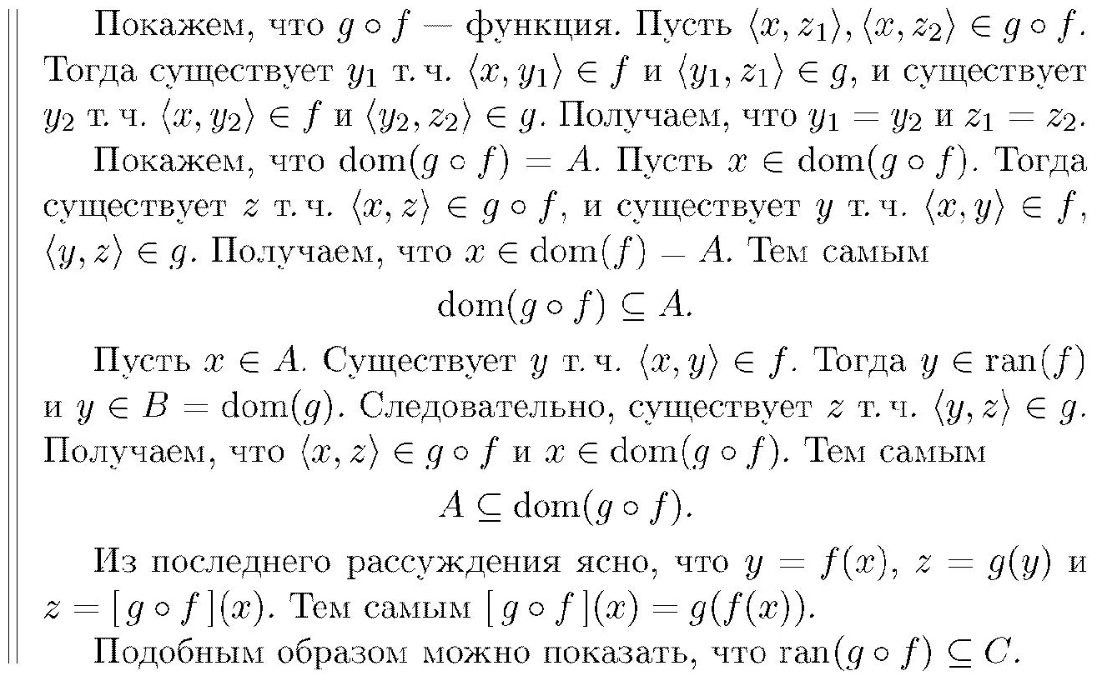
\includegraphics[scale=0.5]{5_1.jpg}\\
 \item Сюръекция, инъекция, биекция, обратная функция, лемма о свойствах биекций
       \\ Пусть $ f: A \rightarrow B$
       \begin{definition*}[Сюръекция]
        $f$ - функция из A \textit{на} B (\textit{сюръективная функция, сюръекция}), если $\forall y \in B$ $\exists x \in A$ | $f(x) = y$
       \end{definition*}
       \begin{name}[Сюръекция]
        $f: A\xrightarrow[\textit{на}]{}B$.
       \end{name}
       \begin{definition*}[Инъекция]
        $f$ - инъективная функция (\textit{1 - 1 функция, инъекция}), если $\forall x_{1}, x_{2}\in A $ из $f(x_{1}) = f(x_{2})$ следует $x_{1} = x_{2}$
       \end{definition*}
       \begin{name}[Инъекция]
        $f: A \xrightarrow{1-1} B$
       \end{name}
       \begin{definition*}[Биекция]
        $f$ - \textit{биекция} из A на B, если $f$ одновременно и инъекция, и сюръекция.
       \end{definition*}
       \begin{name}[Биекция]
        $f: A \xrightarrow[\textit{на}]{1-1} B$
       \end{name}
       \begin{definition*}[Обратная функция]
        Запись $f^{-1}$ означает обратное бинарное отношение к $f$. Если $f^{-1}$ при этом является функцией, то она называется \textit{обратной функцией} к $f$.
       \end{definition*}

       \begin{lemma*}[о свойствах биекций]\mbox{}\\
        \begin{enumerate}
         \item Если $f: A \xrightarrow[\textit{на}]{1-1} B$, то $f^{-1}: B \xrightarrow[\textit{на}]{1-1} A$, $f^{-1}(f(x)) = x$ $\forall x \in A$ и $f(f^{-1}(y)) = y$ $\forall y \in B$.
         \item Если $f: A \xrightarrow[\textit{на}]{1-1} B$, $g: B \xrightarrow[\textit{на}]{1-1} C$, то $g \circ f:  A \xrightarrow[\textit{на}]{1-1} C$.
        \end{enumerate}
       \end{lemma*}


       \begin{proof}
        \begin{enumerate}
         \item Покажем, что $f^{-1}$ - функция.\\ Пусть \mbox{$<y, x_1>, <y, x_2> \in f^{-1}$}. Тогда $<x_1, y>, <x_2, y>\in f$ и $f(x_1) = f(x_2) = y$. Поскольку $f$ инъективна, $x_1 = x_2$.\\
               Ясно, что $dom(f^{-1}) = ran(f)$ и $ran(f^{-1}) = dom(f)$. Поскольку $f$ сюръективна, $ran(f) = B = dom(f^{-1})$. Поскольку $ran(f^{-1}) = A$, $f^{-1}$ сюръективна. Инъективность $f^{-1}$ легко проверяется. Тем самым $f^{-1}: B\xrightarrow[\textit{на}]{1-1} A$.\\
               Покажем, что $f^{-1}(f(x)) = x$ при $x \in A$. Пусть  $x \in A$ и $y = f(x)$. Тогда $<x, y>\in f$ и $<y, x> \in f^{-1}$. Получаем, что $f^{-1}(y) = x$.
         \item выше доказано, что $g \circ f: A \rightarrow C$ и $[g \circ f](x) = g(f(x))$. Инъективность: если $g(f(x_1)) = g(f(x_2))$, то $f(x_1) = f(x_2)$ и отсюда $x_1 = x_2$. Сюръективность доказывается похожим способом.
        \end{enumerate}

       \end{proof}
 \item Отношения эквивалентности, классы эквивалентности, лемма о классах эквивалентности.
       \mbox{}\\ 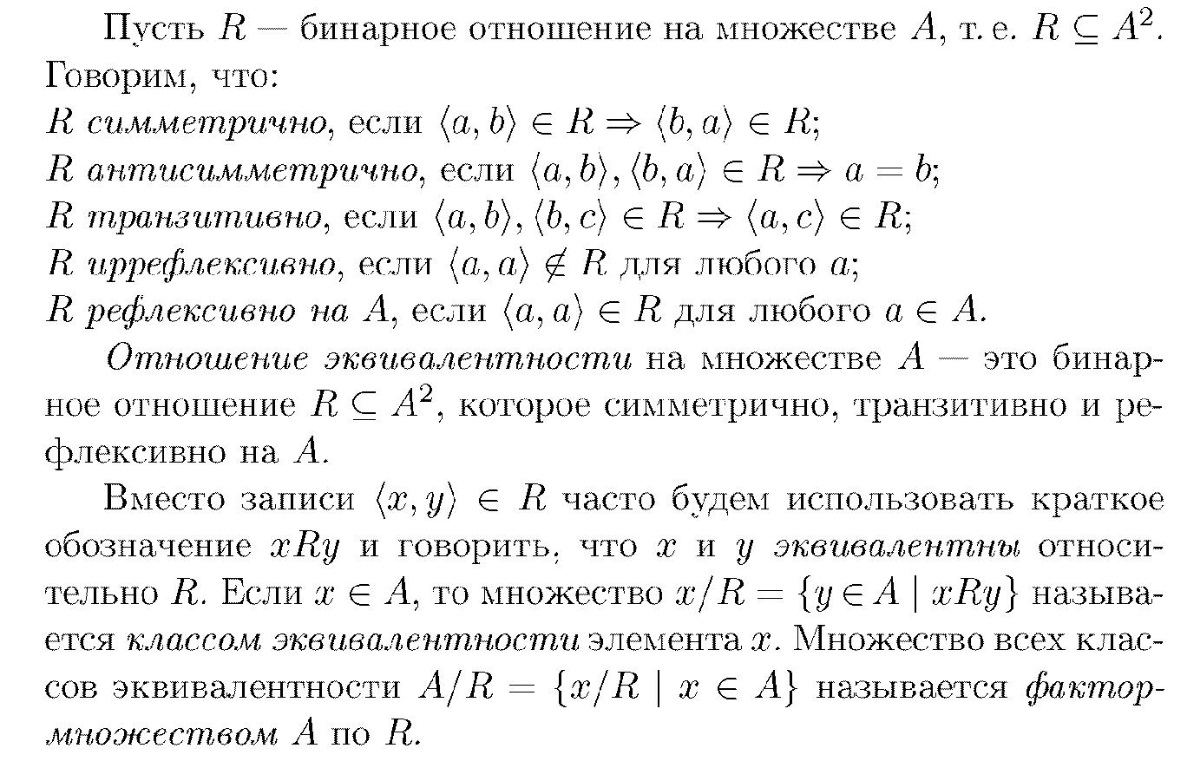
\includegraphics[scale=0.45]{7_1.jpg}\\
       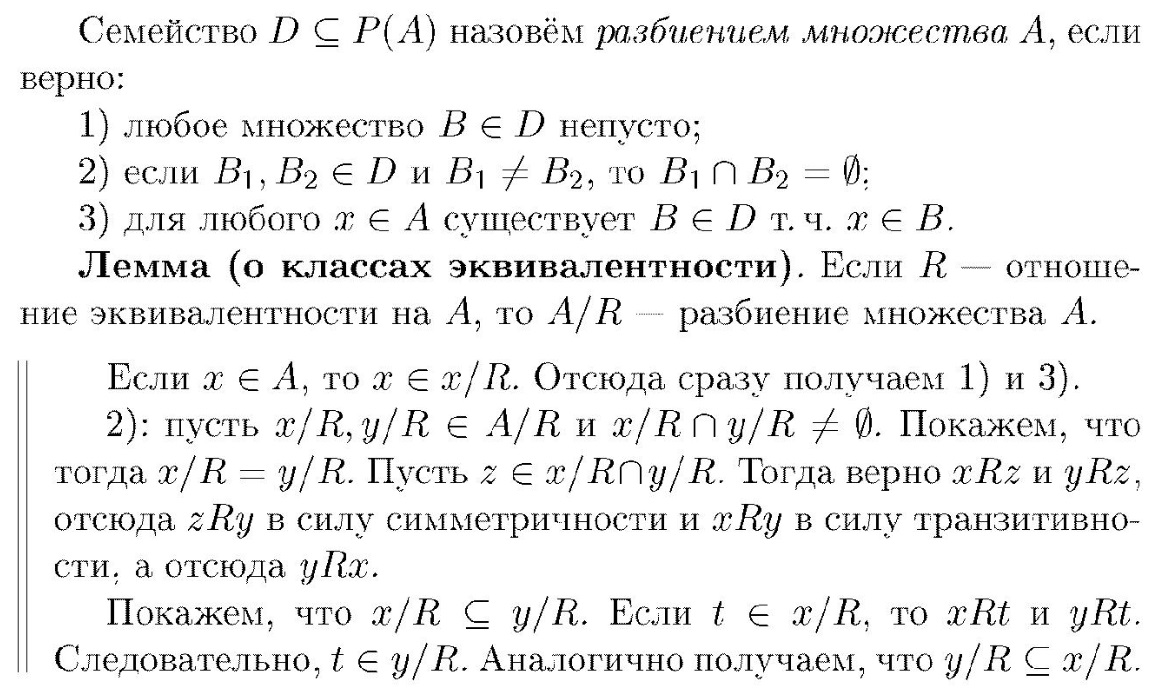
\includegraphics[scale=0.45]{7_2.jpg}
 \item Частичный порядок, ч.у.м., минимальные, максимальные, наименьшие, наибольшие элементы, связи между ними. Замечание о строгом порядке.
       \mbox{}\\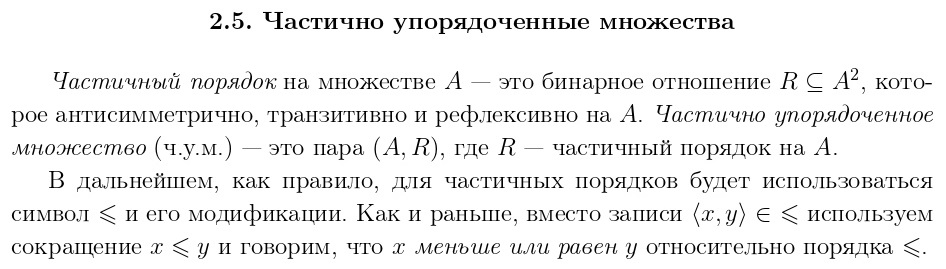
\includegraphics[scale=0.45]{8_1.jpg}\\
       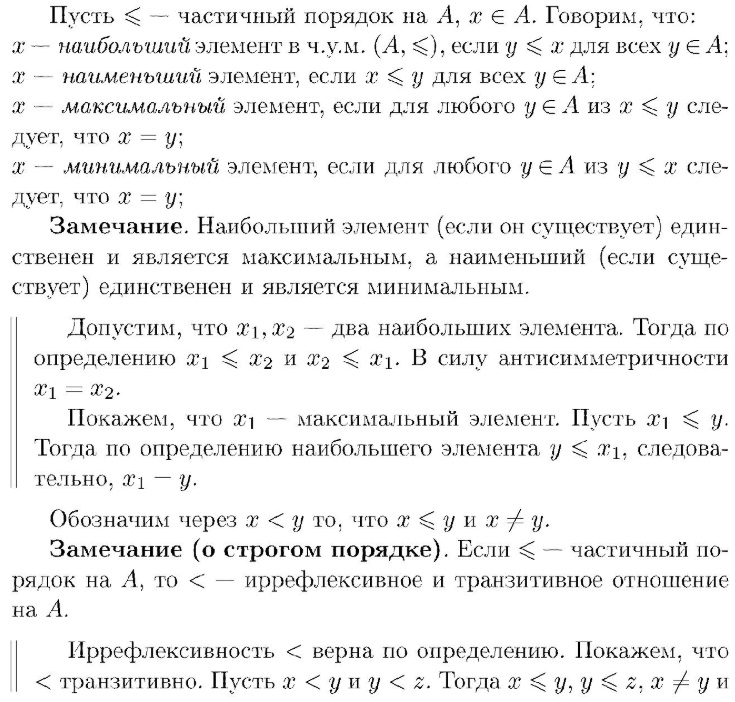
\includegraphics[scale=0.5]{8_2.jpg}\\
       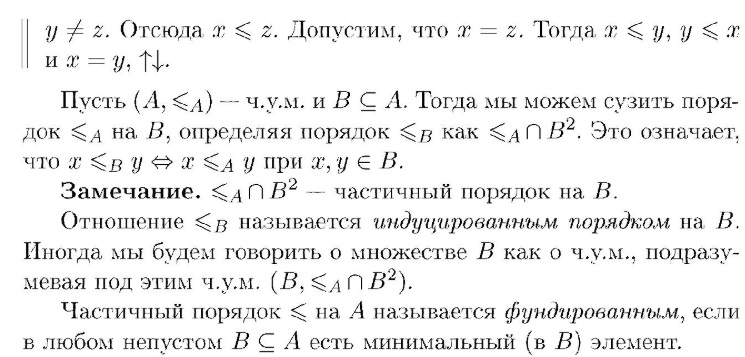
\includegraphics[scale=0.5]{8_3.jpg}
 \item Фундированные частичные порядки, критерий фундированности порядка.
       \mbox{}\\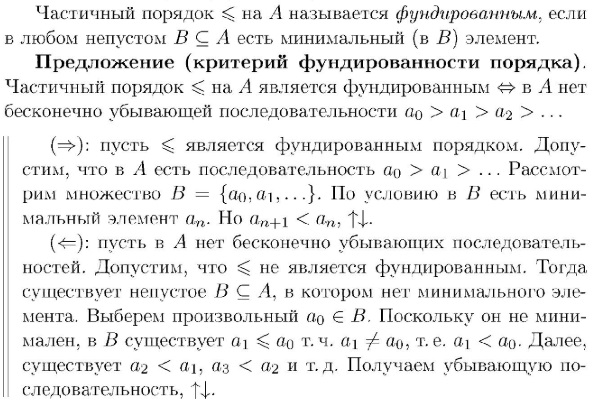
\includegraphics[scale=0.85]{9_1.jpg}\\
 \item Предложение об индукции в фундированном ч.у.м., изоморфизм ч.у.м., замечание об изоморфизме ч.у.м.
       \mbox{}\\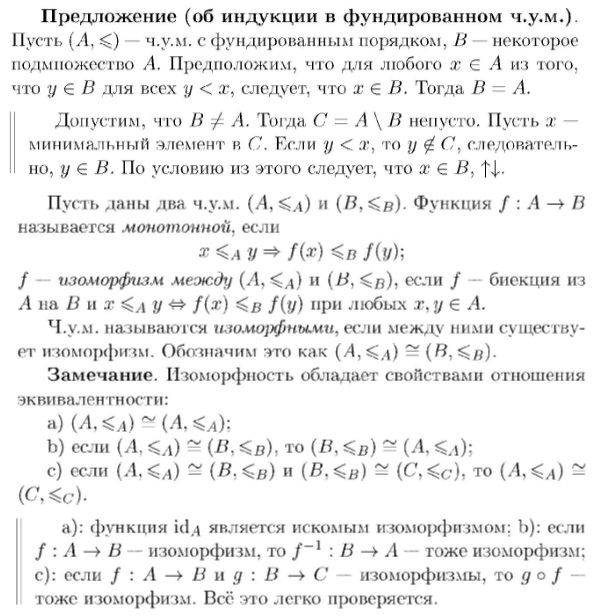
\includegraphics[scale=0.85]{10.jpg}\\
 \item Линейные порядки, л.у.м., начальные сегменты и отрезки, лемма о свойствах начальных сегментов.
       \mbox{}\\ 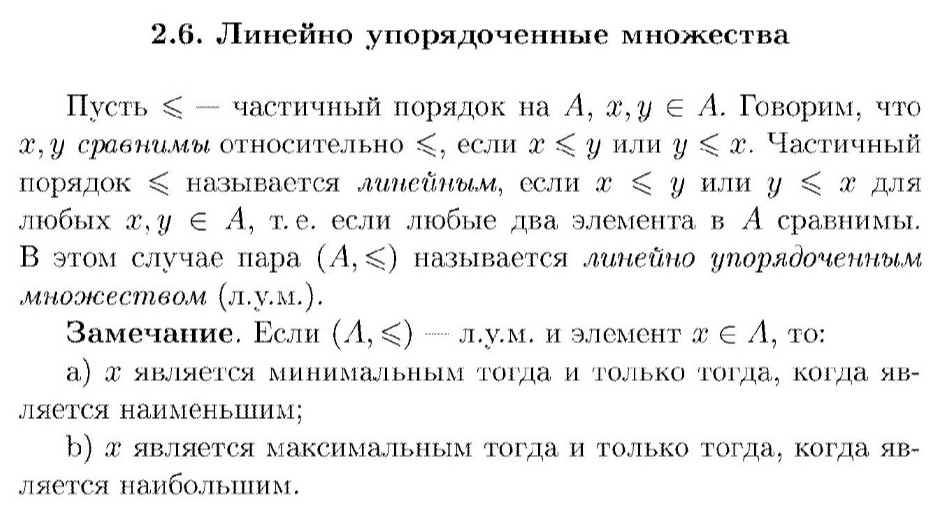
\includegraphics[scale=0.4]{11_1.jpg}\\
       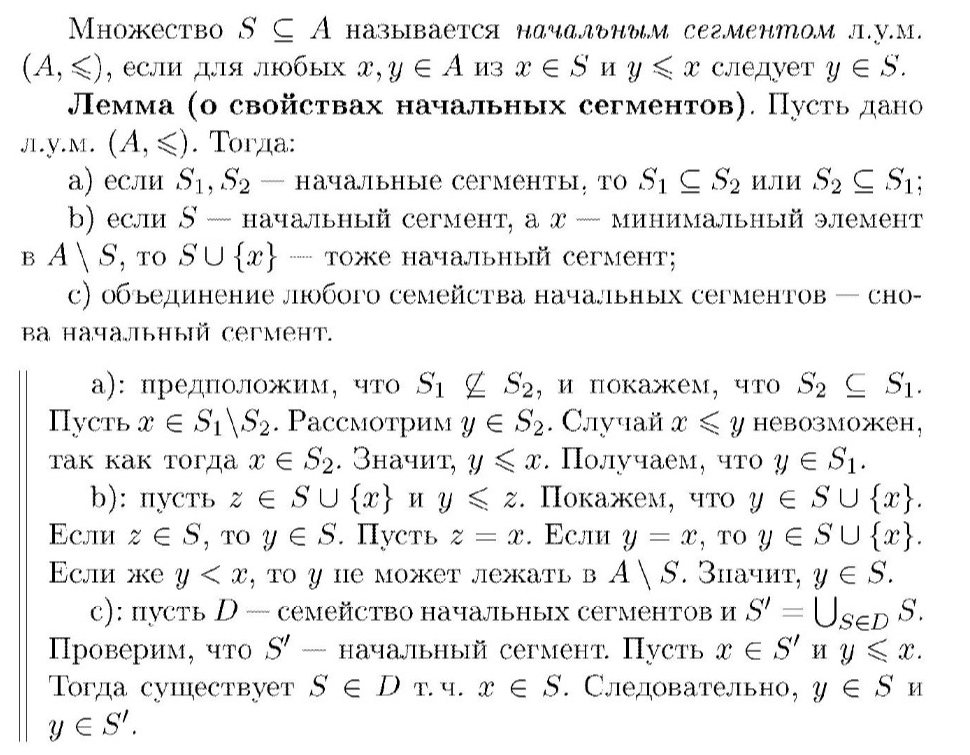
\includegraphics[scale=0.4]{11_2.jpg}\\
       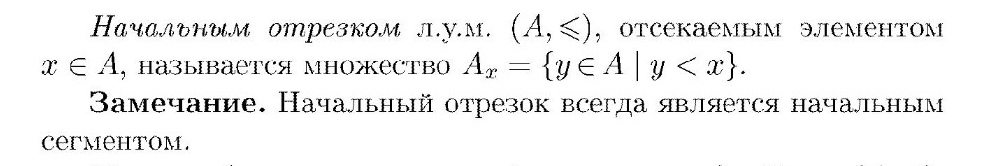
\includegraphics[scale=0.4]{11_3.jpg}
 \item Изоморфизм ч.у.м., изоморфизм л.у.м., признак изоморфизма л.у.м., лемма о монотонной инъекции в.у.м.
       \mbox{}\\ 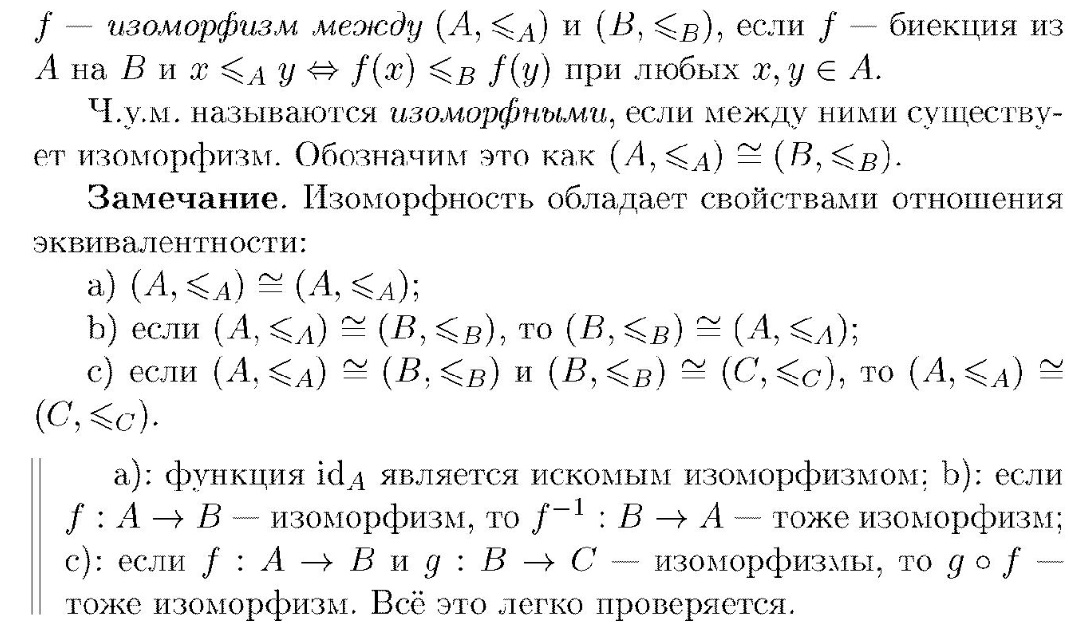
\includegraphics[scale=0.45]{12_1.jpg}\\
       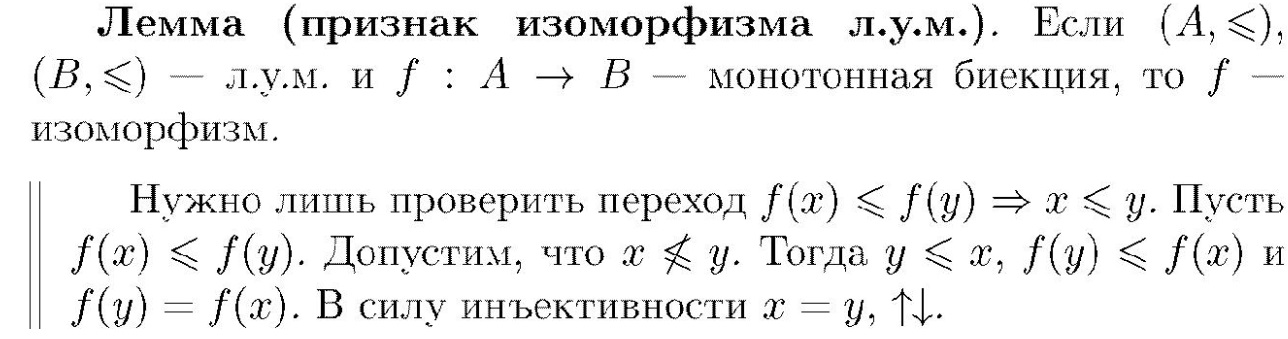
\includegraphics[scale=0.35]{12_2.jpg}\\
       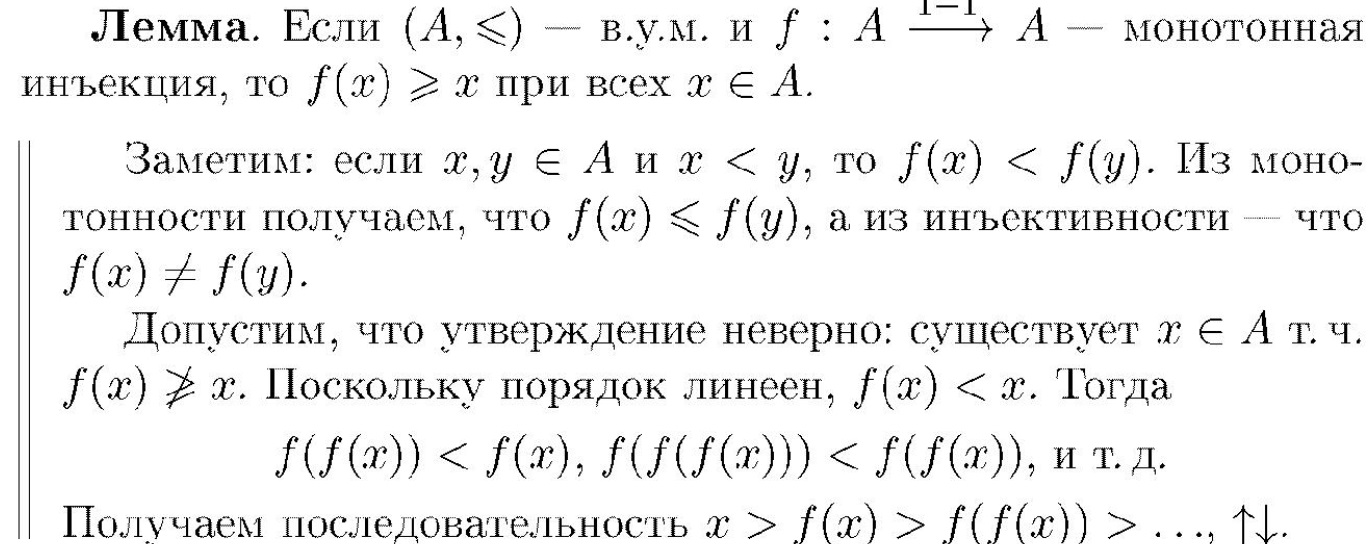
\includegraphics[scale=0.35]{12_3.jpg}
 \item Полный порядок, в.у.м., лемма о начальных сегментах в.у.м.
       \begin{definition*}[Вполне упорядоченное множество]
        \textit{Вполне упорядоченное множество} (в.у.м) - это пара $(A, \leq)$, где $\leq$ - линейный фундированный порядок на $A$. Иногда такой порядок называют \textit{полным}.
       \end{definition*}
       \begin{lemma*}[о начальных сегментах в.у.м.]
        Любой начальный сегмент в.у.м. $(A, \leq)$ либо равен $A$, либо является начальным отрезком.
       \end{lemma*}
       \begin{proof}
        Пусть $S$ - начальный сегмент в $A$ и $S \neq A$. Тогда $A \backslash S \neq \emptyset$. Пусть $x$ - минимальный элемент в $A \backslash S$. Покажем, что $S = A_x$. Если $y \in S$, то либо $y < x$, либо $x \leq y$. Второй случай невозможен, так как тогда $x \in S$.
       \end{proof}
 \item Предложение об изоморфизме начальных сегментов, теорема о сравнимости в.у.м. (без доказательства).
       \begin{proposition*}[об изоморфизме начальных сегментов]
        Различные начальные сегменты в.у.м. не могут быть изоморфны друг другу.
       \end{proposition*}
       \begin{proof}
        Пусть $S_1$ и $S_2$ - два различных сегмента в.у.м. $(A, \leq)$. Тогда сначала докажем лемму о том, что если $(A, \leq)$ - в.у.м. и $f: A \xrightarrow{1-1}A$ - монотонная инъекция, то $f(x) \geq x$ $ \forall x \in A$.\\
        Заметим: если $x, y \in A$ и $x < y$, то $f(x) < f(y)$. Из монотонности получаем, что $f(x) \leq f(y)$, а из инъективности - что $f(x) \neq f(y)$.\\
        Допустим, что утверждение неверно: существует $x \in A$ | $f(x) \ngeqslant x$. Поскольку ряд линеен, $f(x) < x$. Тогда\\$f(f(x))<f(x)$, $f(f(f(x)))<f(f(x))$, и т.д.\\
         Получаем последовательность $x > f(x) > f(f(x)) > ...$, противоречие.\\ \\
         По доказанной лемме $S_1 \subseteq S_2$ или $S_2 \subseteq S_1$. Пусть $S_1 \subseteq S_2$. Выберем $x_0 \in S_2 \backslash S_1$.\\
         Мы рассматриваем эти сегменты как в.у.м. с индуцированным из $A$ порядком. Допустим, что $f: S_2\rightarrow S_1$ - изоморфизм. Рассматривая $f$ как функцию из $S_2$ в $S_2$, видим, что она инъективна и монотонна. Следовательно, $f(x_0) \geq x_0$. Поскольку $S_1$ начальный сегмент и $f(x_0) \in S_1$, получаем, что $x_0 \in S_1$, противоречие.
       \end{proof}
       \begin{theorem*}[о сравнимости в.у.м.]
        Если даны два в.у.м., то одно из них изоморфно начальному сегменту другого.
       \end{theorem*}
 \item Аксиома выбора, лемма Цорна (без доказательства), теорема Цермело (без доказательства), эквивалентность утверждений.
       \begin{flushright}
        \mbox{}\\ 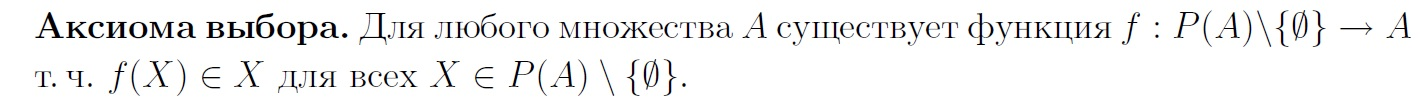
\includegraphics[scale=0.4]{15_1.jpg}\\
        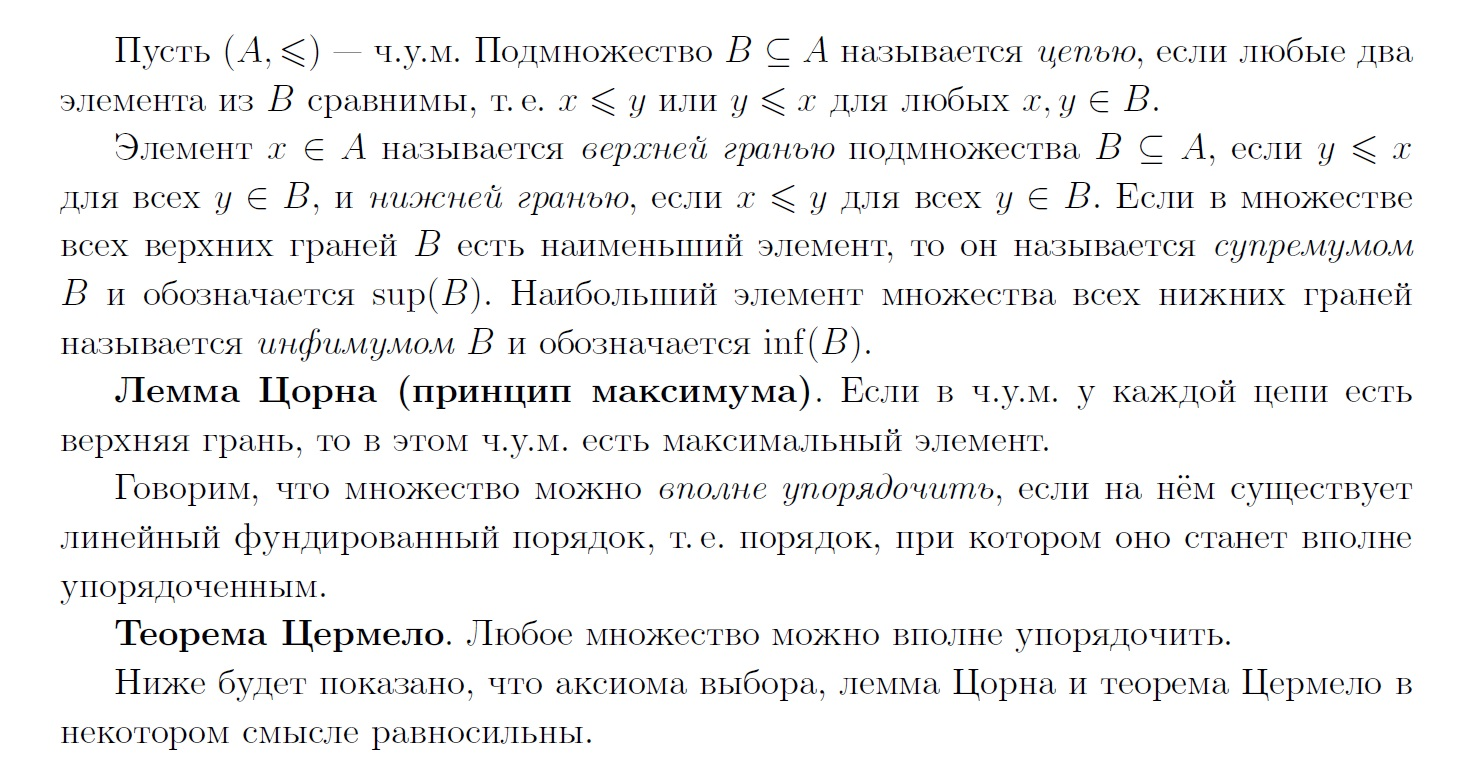
\includegraphics[scale=0.4]{15_2.jpg}\\
       \end{flushright}
 \item Парадокс Рассела, аксиоматика ZFC.
       \begin{paradoks}[Парадокс Рассела]
        Рассмотрим совокупность:
        $M_{R} = \{ A \mid  A$ - множество и $A  \notin A \}$.\\
        Предположим, что само $M_{R}$ является множеством. Возможны два варианта:\\
        \begin{enumerate}
         \item $M_{R} \notin{M_{R}}$. Тогда $A - M_{R}$ подходит под определние, и $M_{R} \notin{M_{R}}$. Противоречие.
         \item $M_{R} \in{M_{R}}$. Вновь полагая, $A = M_{R}$, получаем, что по определению $M_{R} \notin{M_{R}}$. Противоречие.
        \end{enumerate}
        Это рассуждение показывает, что совокупность $M_{R}$ нельзя считать множеством.
       \end{paradoks}
       Аксиоматика ZFC.\\
       Можно с собой на листочке!!!
 \item Равномощные множества, замечание о равномощности.
       \begin{name}[мощность множества]
        Мощность множества $A$ обозначается $|A|$.
       \end{name}
       \begin{definition*}[равномощные множества]
        Говорим, что множества $A$ и $B$ равномощные, если существует биекция $f: A \xrightarrow[ \text{на}]{1-1} B$. \\
        Обозначим это символической записью $|A| = |B|$.
       \end{definition*}
       \begin{comment*}[о равномощности]
        Равномощность обладаает свойствами отношения эквивалентности - для любых множеств $A, B, C$ верно:
        \begin{enumerate}
         \item $|A| = |A|$;
         \item $|A| = |B| \Rightarrow |B| = |A|$;
         \item $|A| = |B|$ и $|B| = |C| \Rightarrow |A| = |C|$;
        \end{enumerate}
       \end{comment*}
       \begin{proof}
        Следует из леммы о свойствах биекций.
       \end{proof}
 \item Лемма о порядке на мощностях.
       \begin{lemma*}[Лемма о порядке на мощностях]
        Для всяких непустых множеств $A$ и $B$ следующие условия эквиваленты:
        \begin{enumerate}
         \item $\left | A \right | \leq \left | B \right |$
         \item Существует функция $g : B\xrightarrow[\textit{на}]{}A$
         \item $A$ равномощно некоторому подмножеству $B$
        \end{enumerate}
       \end{lemma*}
       \begin{proof}
        \mbox{}\\
        \begin{enumerate}
         \item $a \Rightarrow c$ \\
               Пусть $\left | A \right | \leq \left | B \right |$.\\
               Тогда существует $f : A \xrightarrow[]{1-1} B$. \\
               Тогда $ran(f) \subseteq B$ и $f : A\xrightarrow[\textit{на}]{1-1}ran(f)$.\\
         \item $c \Rightarrow b$ \\
               Пусть $h : B_{1}\xrightarrow[\text{на}]{1-1}A$, где $B_{1}\subseteq B$. \\
               Выберем произвольное $a_{0} \in A$ и построим $g : B\xrightarrow[\text{на}]{}A$ так:
               $g(y) = \left\{\begin{matrix}
                 h(y)\text{, если } y \in B_{1} \\
                 a_{0}\text{, если }y \in B\backslash B_{1}
                \end{matrix}\right.$
         \item $b \Rightarrow a$ \\
               Пусть $g : B\xrightarrow[\text{на}]{ }A$.\\
               Построим $f : B\rightarrow A$.\\
               Рассмотрим $x\in A$\\
               Множество $\{y\in B |\ g(y) = x\}$ непусто.\\
               Выберем в качестве $f(x)$ некоторый элемент из этого множества. Проверим, что $f$ инъективна. Пусть $f(x_{1}) = f(x_{2})$\\
               Тогда $g(f(x_{1})) = g(f(x_{2}))$ , а по построению $g(f(x_{i})) = x_{i}$ при $i = 1,2.$
        \end{enumerate}
       \end{proof}
 \item Теорема Кантора-Бернштейна.
       \mbox{}\\ 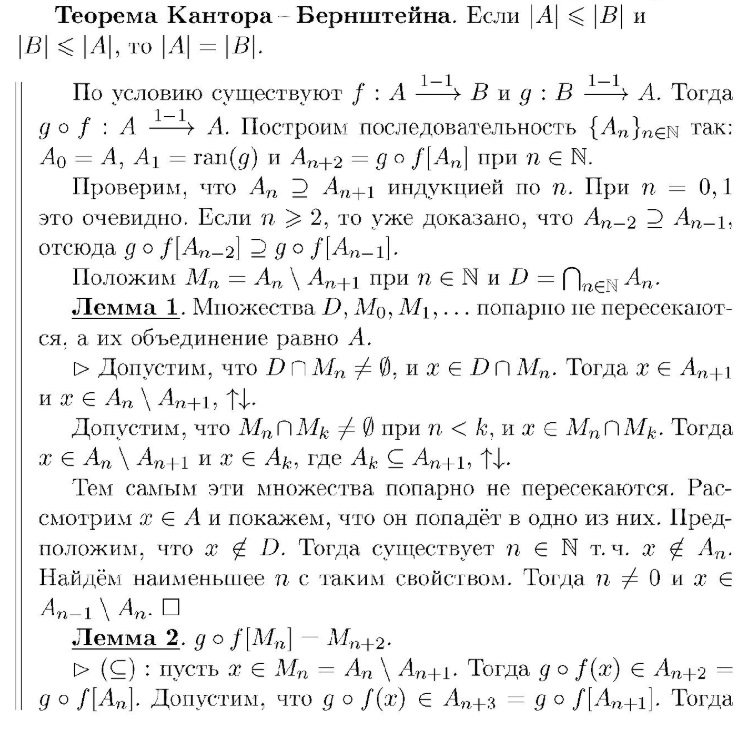
\includegraphics[scale=0.7]{19_1.jpg}\\
       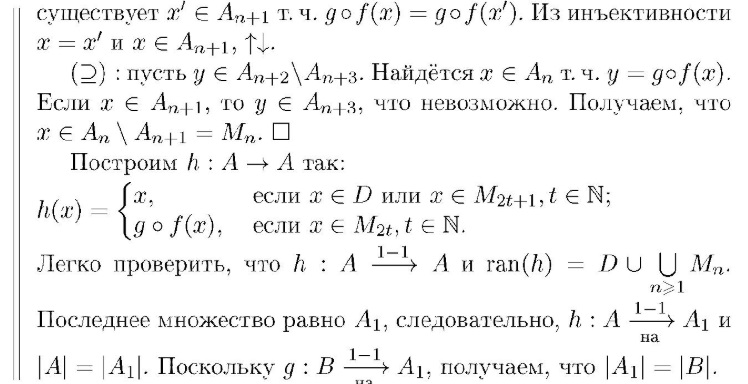
\includegraphics[scale=0.7]{19_2.jpg}
 \item Теорема о сравнимости мощностей, теорема Кантора.
       \mbox{}\\ 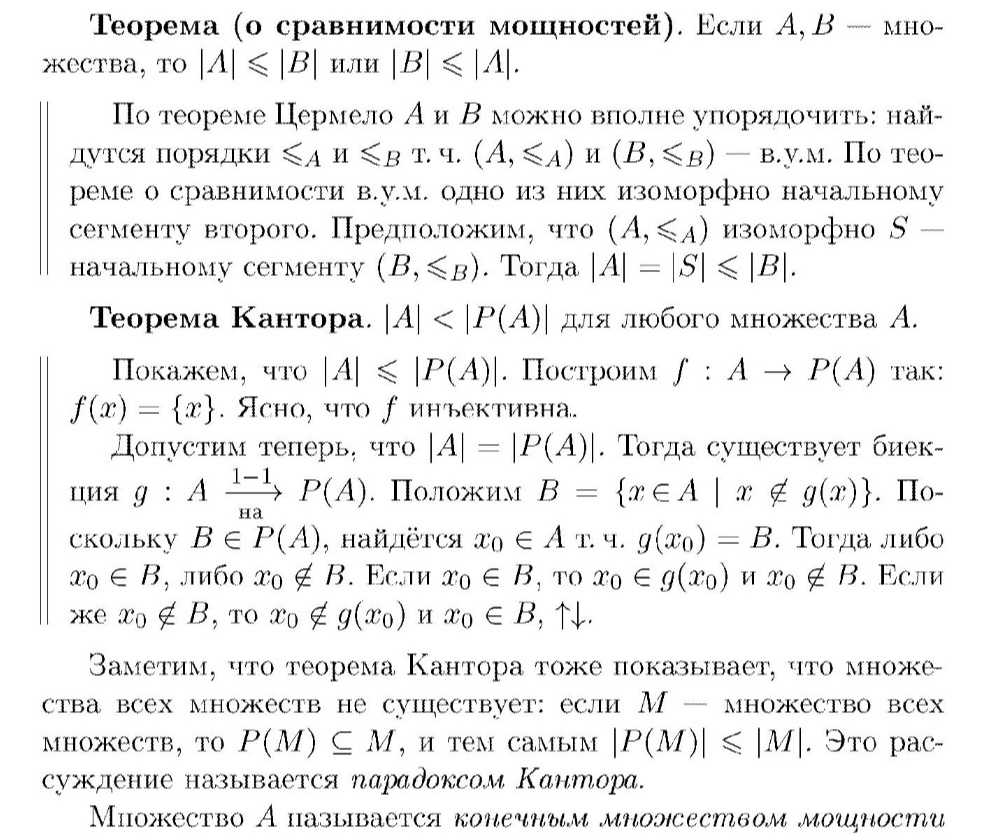
\includegraphics[scale=0.4]{20_1.jpg}\\
       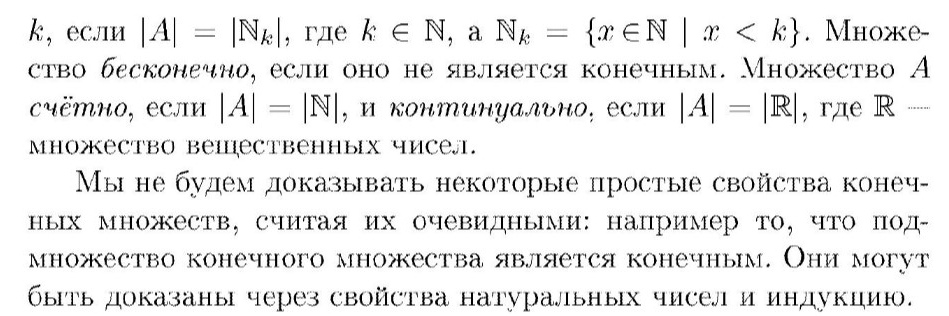
\includegraphics[scale=0.4]{20_2.jpg}\\
 \item Конечные, бесконечные, счетные, континуальные множества, описание не более чем счетных множеств.
       \begin{definition*}[Конечное множество]
        Множество $A$ называется \textit{конечным множеством мощности $k$}, если $|A| = |\mathbb{N}_k|$, где $k \in \mathbb{N}$, а $\mathbb{N}_k = \{x \in \mathbb{N} | x < k\}$
       \end{definition*}
       \begin{definition*}[Бесконечное множество]
        Множество \textit{бесконечно}, если оно не является конечным.
       \end{definition*}
       \begin{definition*}[Счётное множество]
        Множество $A$ \textit{счётно}, если $|A| = |\mathbb{N}|$.
       \end{definition*}
       \begin{definition*}[Континуальное множество]
        Множество $A$ \textit{континуально}, если $|A| = |\mathbb{R}|$.
       \end{definition*}
       \begin{definition*}[Не более чем счётное множество]
        Множество $A$ \textit{не более чем счётно}, если $|A| \leq |\mathbb{N}|$
       \end{definition*}
       \begin{consequence*}[Описание не более чем счётных множеств]
        Множество не более чем счётно тогда и только тогда, когда оно конечно или счётно.
       \end{consequence*}
       \begin{proof}
        $\Leftarrow$: счётное множество не более чем счётно. Если $A$ конечно, то $|A| = |\mathbb{N} _k|\leq |\mathbb{N}|$. \\
        $\Rightarrow$: Пусть $A$ не более чем счётно. Предположим, что оно бесконечно. Тогда в $A$ есть счётное подмножество $B$. Получаем, что $|\mathbb{N}| - |B| \leq |A| \leq |\mathbb{N}|$. По теореме Кантора-Бернштейна $|A| = |\mathbb{N}|$.
       \end{proof}
 \item Лемма о сохранении мощностей, теорема о мощности объединения (без доказательства).
       \begin{lemma*}[Лемма о сохранении мощностей]\mbox{}\\
        \begin{enumerate}
         \item Если $\left | A \right | = \left | A_{1} \right |$ и $\left | B \right | = \left | B_{1} \right |$, то $\left | A\times B \right | = \left | A_{1}\times B_{1} \right |$\\
         \item Если при этом $A\cap B = A_{1}\cap B_{1}=\emptyset $, то $\left | A \cup B \right | =\left | A_{1} \cup B_{1} \right |  $
        \end{enumerate}
       \end{lemma*}
       \begin{proof}\mbox{}\\
        \begin{enumerate}
         \item Пусть даны биекции \\$f : A\xrightarrow[\text{на}]{1-1}A_{1}$ и $g : B\xrightarrow[\text{на}]{1-1}B_{1}$.\\
                Построим $h : A \times B\xrightarrow[\text{на}]{1-1}A_{1} \times B_{1}$ так:
               $h_{1}(<x;y>)=<f(x),g(y)>$.
                Легко проверить, что $h_{1}$ - нужная биекция.
         \item Построим $h_{2} : A\cup B \xrightarrow[\text{на}]{1-1}A_{1}\cup B_{1}$ так:
               $h_{2}(x) =
                \left\{
                \begin{matrix}
                 f(x)\text{, если } x \in A \\
                 g(x)\text{, если } x \in B \\
                \end{matrix}
                \right.$
               Условие $A \cap B = \emptyset$ гарантирует, что определение корректно.
               Вновь нетрудно доказать, что $h_{2}$ - биекция. Проверим в качестве примера, что $h_{2}$ инъективна. Пусть $h_{2}(x)=h_{2}(y)$. Если $x,y \in A$, то получаем $f(x)=f(y)$ и $x=y$. Если $x,y \in B$, рассуждения аналогичны. Если же $x \in A, y \in B$  (или наоборот), то $h_{2}(x) \in A_{1}$ и $h_{2}(y) \in B_{1}$, что невозможно в силу $A_{1} \cap B_{2} = \emptyset$.
        \end{enumerate}
       \end{proof}
       \begin{lemma*}[о мощности объединения] Если хотя бы одно из множеств $A,B$ бесконечно, то $\left | A \cup B \right | = max\{\left | A \right |,\left | B \right |\}$.
       \end{lemma*}
 \item Теорема о мощности квадрата бесконечного множества (доказательства для счетного и континуального), теорема о мощности произведения (без доказательства).
       \begin{theorem*}[о мощности квадрата бесконечного множества]
        Если $A$ - бесконеное множество, то $|A\times{A}|=|A|$
       \end{theorem*}
       \begin{proof}\mbox{}\\
        \begin{itemize}
         \item Докажем, что $|\mathbb {N} \times{\mathbb{N}|} = |\mathbb {N}|$
               \\Построим $f: \mathbb{N}\times{\mathbb{N}} \xrightarrow[]{1-1}{\mathbb{N}}$ и $g: \mathbb{N}\xrightarrow[]{1-1}{\mathbb{N}\times{\mathbb{N}}}$
               \\ $f(x,y) = 2^x+3^y$
               \\ $g(x) = <x, 0>$
               \\ Заметим, что обе функции инъективны, а значит $\left\{
                \begin{matrix}
                 |\mathbb {N} \times{\mathbb{N}|} \leq |\mathbb {N}| \\
                 |\mathbb {N} \times{\mathbb{N}|} \geq |\mathbb {N}| \\
                \end{matrix}
                \right.$
               тогда по теореме \textit{Кантора-Бернштейна} получаем, что $|\mathbb {N} \times{\mathbb{N}|} = |\mathbb {N}|$
         \item Докажем, что $|\mathbb{R} \times{\mathbb{R}|} = |\mathbb{R}|$\\
               По аналогии с $\mathbb{N}$ построим две инъекции: \\
               \begin{enumerate}
                \item $f: \mathbb{R}\times{\mathbb{R}} \xrightarrow[]{1-1}{\mathbb{R}}$
                      \\Для построения данной функции докажем, равномощность $\mathbb{R}$ и $(0,1)$:\\
                      Для этого построим биекцию $h: (0,1) \xrightarrow[\text{на}]{1-1} \mathbb{R}$
                      \\ $h(x) = ctg(x*\pi)$ - функция биекция из-за $E(ctg x) = \mathbb{R}$\\
                      Значит $|\mathbb{R}| = |(0,1)|$
                      \\Докажем, что $\mathbb{R}\times{\mathbb{R}}$ равномощно $(0,1)\times(0,1)$:
                      \\ Для этого построим $w: (0,1)\times(0,1)\xrightarrow[\text{на}]{1-1} \mathbb{R}\times{\mathbb{R}}$
                      \\ $w(x,y)=<h(x), h(y)>$\\
                      Значит $|\mathbb{R}\times{\mathbb{R}}| = |(0,1)\times(0,1)|$
                      \\ Построим инъекцию $u: (0,1)\times(0,1)\xrightarrow[]{1-1}(0,1)$
                      \\$u(x,y)=0,\frac{10*a_1}{2}\frac{10*b_1}{2}\frac{10*a_2}{2}\frac{10*b_2}{2}...$\\
                       Где $x = 0,a_{1}a_{2}...$, а $y=0,b_{1}b_{2}...$
                       \\ Т.к в формуле присутсвует умножение на 10, то на каждое число из $\frac{10*a_1}{2}\frac{10*b_1}{2}\frac{10*a_2}{2}\frac{10*b_2}{2}...$ отводится по две цифры, т.е $\frac{10*4}{2} = 20$, а $\frac{10*9}{2}=45$, также $\frac{10*0}{2}=00$
                       \\ $u$ - инъекция, тогда $f(x,y)=h\circ{u}\circ{w^{-1}}(x,y)$
                \item $g: \mathbb{R}\xrightarrow[]{1-1}{\mathbb{R}\times{\mathbb{R}}}$
                      \\ Построим $g(x) = <x,0>$
               \end{enumerate}
               Т.к $f$ и $g$ - инъекции, значит значит $\left\{
                \begin{matrix}
                 |\mathbb {R} \times{\mathbb{R}|} \leq |\mathbb {R}| \\
                 |\mathbb {R} \times{\mathbb{R}|} \geq |\mathbb {R}| \\
                \end{matrix}
                \right.$
               тогда по теореме \textit{Кантора-Бернштейна} получаем, что $|\mathbb {R} \times{\mathbb{R}|} = |\mathbb {R}|$
        \end{itemize}
       \end{proof}
       \begin{theorem*}[о мощности произведения]
        Если $A, B$ - непустые множества и одно из них бесконечно, то: \\$|A\times{B}| = max\{|A|, |B|\}$
       \end{theorem*}
 \item Континуум-гипотеза, теорема Гёделя-Коэна (без доказательства), обобщенная континуумгипотеза.
       \begin{hypo}[Континуум-гипотеза] Не существует множества $A$ такого, что\\
        $\left | \mathbb{N} \right | < \left | A \right | < \left | \mathbb{R} \right |$
       \end{hypo}
       \begin{theorem*}[Теорема Гёделя-Коэна]
        Если теория множеств ZFC непротиворечива, то континуум-гипотезу нельзя ни доказать, ни опровергнуть в рамках ZFC.
       \end{theorem*}
       \begin{hypo}[Обобщенная континуумгипотеза]
        Если множество $B$ - бесконечно, то не существует множества $A$ такого, что\\ $\left | B \right | < \left | A \right | < \left | P(B) \right |$
       \end{hypo}
 \item Ординалы, лемма об элементах ординала
       \begin{definition*}[Ординал]
        Ординалом называется транзитивное множество все элементы которого сравнимы относительно включения.
       \end{definition*}
       \begin{definition*}[Транзитивное множество]
        Множество $\alpha$ называется транзитивным, если из $x \in \alpha $ и $y \in x $ следует, что  $y \in \alpha $.
       \end{definition*}
       \begin{lemma*}[Лемма об элементах ординала]
        Если $\alpha$ - ординал и $\beta \in \alpha$, то $\beta$ - ординал.
       \end{lemma*}
       \begin{proof}
        Пусть $x,y\in \beta$. Тогда $x,y\in \alpha$. Следовательно, $x$ и $y$ равны или сравнимы относительно $\in$. Докажем, что $\beta$ транзитивно. Пусть $y \in x \in \beta$. Тогда $x \in \alpha$ и $y \in \alpha$. Возможны три случая:
        \begin{enumerate}
         \item $\beta \in y$ Тогда получаем, что $\beta \in y \in x \in \beta$ - противоречие.
         \item $\beta = y$ Получаем, что $\beta \in x \in \beta$ - противоречие.
         \item $y \in \beta$.
               Следовательно, $\beta$ - ординал.
        \end{enumerate}
       \end{proof}
 \item Лемма о порядке на ординалах, теорема о свойствах ординалов.
       \begin{lemma*}[о порядке на ординалах]
        Для любых ординалов $\alpha, \beta$ равносильно:
        \begin{enumerate}
         \item $\alpha \leq \beta$;
         \item $\alpha \subseteq \beta$.
        \end{enumerate}
       \end{lemma*}
       \begin{proof}
        (a $\Rightarrow$ b): если $\alpha = \beta$, то $\alpha \subseteq \beta$. Если же $\alpha \in \beta$ и $x \in \alpha$, то $x \in\beta$\\
        (b $\Rightarrow$ a): если $\alpha = \beta$ , то $\alpha \leq \beta$. Предположим, что $\alpha \subset \beta$. Тогда $\beta \backslash \alpha \neq \emptyset$. По аксиоме регулярности $\exists \gamma \in \beta \backslash \alpha$ т. ч. $\gamma \cap (\beta \backslash \alpha) \neq \emptyset$. Покажем, что $\alpha = \gamma$. \\
        Если $x \in \gamma$, то $x \in \beta$ и $x \notin \beta \backslash \alpha$, следовательно, $x\in \alpha$. \\
        Если $x \in \alpha$, то $x \in \beta$ и возможны три случая:
        \begin{enumerate}
         \item $\gamma \in x$. Тогда $\gamma \in \alpha$, противоречие.
         \item $\gamma = x$. Вновь $\gamma \in \alpha$, противоречие.
         \item $x \in \gamma$.
        \end{enumerate}
        Получаем, что $\alpha \in \beta$ и $\alpha \leq \beta$.
       \end{proof}

       \begin{theorem*}[о свойствах ординалов]
        Класс ординалов с порядком $\leq$ обладает свойствами в.у.м. - для любых ординалов $\alpha, \beta, \gamma$ верно:
        \begin{enumerate}
         \item $\alpha \leq \alpha$;
         \item $\alpha \leq \beta$ и $\beta \leq \alpha \Rightarrow \alpha = \beta$;
         \item $\alpha \leq \beta$ и $\beta \leq \gamma \Rightarrow \alpha \leq \gamma$;
         \item $\alpha \leq \beta$ или $\beta \leq \alpha$;
         \item в любом непустом множестве ординалов есть минимальный элемент.
        \end{enumerate}
       \end{theorem*}

       \begin{proof}
        \begin{enumerate}
         \item очевидно.
         \item если $\alpha \subseteq \beta$ и $\beta \subseteq \alpha$, то $\alpha = \beta$.
         \item если $\alpha \subseteq \beta$ и $\beta \subseteq \gamma$, то $\alpha \subseteq \gamma$.
         \item пусть $\delta = \alpha \cap \beta$. Легко проверить, что $\delta$ является ординалом. По лемме о порядке на ординалах $\delta \leq \alpha$ и $\delta \leq \beta$. Если $\delta = \alpha$ или $\delta = \beta$, утверждение доказано. Допустим, что $\delta \neq \alpha, \beta$. Тогда $\delta \in \alpha, \delta \in \beta$ и $\delta \in \alpha \cap \beta = \delta$, противоречие.
         \item пусть $S$ - непустое множество ординалов. По аксиоме регулярности $\exists \alpha \in S$, т.ч. $\alpha \cap S = \emptyset$. Если $\beta < \alpha$, то $\beta \in \alpha$ и $\beta \notin S$. Ясно, что $\alpha$ - минимальный элемент в $S$.
        \end{enumerate}
       \end{proof}
 \item Предложение о супремуме множества ординалов (без доказательства), теорема о связи в.у.м. и ординалов (без доказательства), предложение о принципе трансфинитной индукции (без доказательства).
       \begin{proposition*}[о супремуме множества ординалов]
        Пусть $A$ - некоторое множество ординалов. Тогда $\cup A$ - ординал, являющийся супремумом множества $A$.
       \end{proposition*}
       \begin{theorem*}[о связи в.у.м. и ординалов]
        Для любого в.у.м. существует единственный изоморфный ему ординал.
       \end{theorem*}
       \begin{proposition*}[о трансфинитной индукции]
        Пусть $\Phi(x)$ - некоторое условие. Пусть для любого ординала $\alpha$ из того, что $\Phi(\beta)$ верно для всех $\beta < \alpha$, следует, что верно $\Phi(\alpha)$. Тогда $\Phi(\alpha)$ верно для всех ординалов $\alpha$.
       \end{proposition*}
 \item Сумма и произведение ординалов, кардинал, мощность множества.
       \begin{proposition*}[принцип трансфинитной рекурсии]
        Пусть существует условие, которое для каждого ординала $\alpha$ однозначно задаёт некоторое множество $f_\alpha$ в предположении, что при $\beta < \alpha$ множества $f_\beta$ уже определены. Тогда каждому ординалу $\alpha$ действительно можно сопоставить множество $f_\alpha$ так, чтобы указанная связь между $f_\alpha$ и $f_\beta$, $\beta < \alpha$ выполнялась. При этом $f_\alpha$ определено однозначно.
       \end{proposition*}

       \begin{exmp}
        На классе ординалов можно задать операции + и $\cdot$ так, что для любых ординалов $ \alpha, \beta$ будет верно:
        \begin{enumerate}
         \item $\alpha + 0 = \alpha$ и $\alpha \cdot 0 = 0$;
         \item $\alpha + (\beta + 1) = (\alpha + \beta) + 1$ и $\alpha \cdot (\beta + 1) = (\alpha \cdot \beta) + \alpha$;
         \item $\alpha + \lambda = \sup\{ \alpha + \beta | \beta < \lambda\}$ и $\alpha \cdot \lambda = \sup\{\alpha \cdot \beta | \beta < \lambda\}$, если $\lambda$ - предельный ординал.
        \end{enumerate}
       \end{exmp}
       \begin{proof}
        Зафиксируем $\gamma$ и определим $\gamma + \alpha$ трансфинитной рекурсией по $\alpha$. Предположим, что при $\beta < \alpha$ ординал $\gamma + \beta$ уже определён. Определим $\gamma + \alpha$, просто повторив формулировку для трёх случаев:
        \begin{enumerate}
         \item $\alpha = 0$, тогда $\gamma + \alpha = \gamma$;
         \item $\alpha = \beta + 1$, тогда $\gamma + \alpha =  (\gamma + \beta) + 1$;
         \item $\alpha$ - предельный, тогда $\gamma + \alpha = \sup\{\gamma + \beta | \beta < \alpha\}$.
        \end{enumerate}
        Произведение $\gamma \cdot \alpha$ определяется аналогично.
       \end{proof}

       \begin{definition*}[Кардинал]
        Ординал $\mu$ называется \textit{кардиналом}, если он не равномощен никакому строго меньшему ординалу.
       \end{definition*}

       \begin{definition*}[Мощность множества]
        \textit{Мощность} множества $A$ - это единствееный кардинал, равномощный $A$, т.е. $|\mu_A|=|A|$.
       \end{definition*}
 \item Алфавит ИВ, формула ИВ, подформула, представление формул ИВ.
       \\ Алфавит ИВ состоит из трёх частей:
       \begin{enumerate}
        \item Пророзициональные символы (Заглавные буквы латинского алфавита, возможно, с индексами); \\
        \item Логические связки:\\
              $\lnot\ $- отрицание\\
              $\land\ $- конъюнкция\\
              $\lor\ $- дизъюнкция\\
              $\rightarrow\ $- импликация\\
        \item Вспомогательные символы (запятая $"$$,$$"$);
       \end{enumerate}
       Формула исчисления высказываний:
       \begin{enumerate}
        \item Пропозициональная переменная (Она же - атомарная формула);
        \item Если $A$ и $B$ - формулы, то $\lnot A, (A\land B), (A \lor B), (A \Rightarrow B)$ - формулы.
        \item Других формул нет.
       \end{enumerate}
       \begin{definition*}[Подформула формулы $A$]
        Подформула формулы $A$ - любое подслово слова А, которое само является формулой.
       \end{definition*}
       Пусть $\Delta(n)$ - некоторое высказывание, которое для любого $n$ принимает значение истина или ложь.

       \begin{proposition*}[о представлении формул исчисления высказываний]
        Всякая неатомарная формула исчисления высказываний единственным образом представима в одном из следующих видов:
        \begin{itemize}
         \item $\lnot\Phi$;
         \item $(\Phi \land \Psi)$;
         \item $(\Phi \lor \Psi)$;
         \item $(\Phi \Rightarrow \Psi)$
        \end{itemize}
        Для некоторых $\Phi$ и $ \Psi$.
       \end{proposition*}
 \item Принцип математической индукции и возвратной индукции.
       \begin{definition*}[Принцип математической индукции]
        Если $\Delta(0)$ истинно и для всех $n$ из истинности $\Delta(n)$ следует истинность $\Delta(n + 1)$, то $\Delta(n)$ истинно для всех $n$.
       \end{definition*}

       \begin{definition*}[Возвратная индукция]
        Пусть для каждого $n$ из того, что $\Delta(k)$ истинно при любом $k < n$, следует, что истинно $\Delta(n)$. Тогда $\Delta(n)$ истинн для всех $n$.
       \end{definition*}

       \begin{proof}
        Оба принципа индукции легко вытекают из следующего факта: в любом непустом множестве натуральных числе есть минимальный элемент. Покажем, как отсюда выводится возвратная индукция. \\
        Допустим, что $\Delta(n)$ ложно при некотором $n$. Рассмотрим множество $A = \{n | \Delta(n) \text{ ложно} \}$. Оно не пусто, следовательно, в нём есть минимальный элемент $n_0$. Тогда $\Delta(n_0)$ ложно, а если $n < n_0$, то $n \notin A$ и $\Delta(n)$ истинно. Получаем, что $\Delta(n_0)$ тоже истинно, противоречие.
       \end{proof}
 \item Алфавит ИС, секвенция, аксиома, правило вывода, дерево вывода, доказуемость, пример вывода.
       \mbox{}\\ 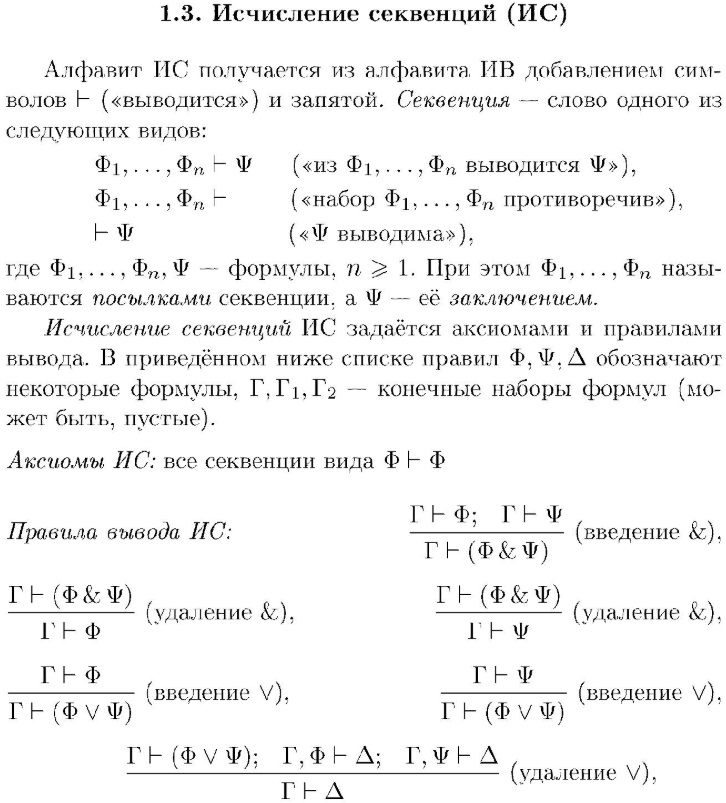
\includegraphics[scale=0.7]{31_1.jpg}\\
       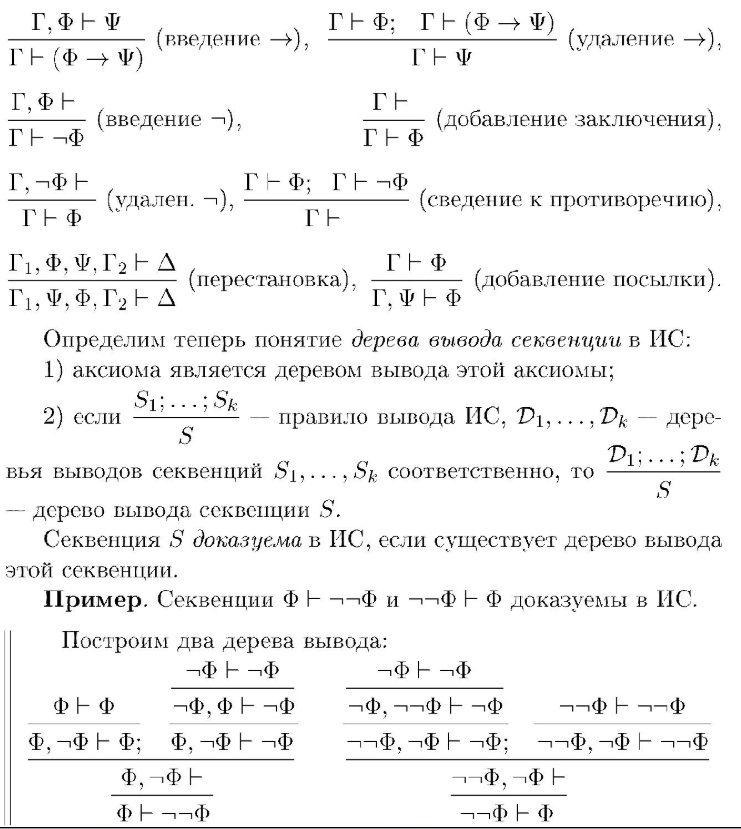
\includegraphics[scale=0.65]{31_2.jpg}
 \item Семантика ИВ: означивание, значение формулы при означивании, выполнимые, опровержимые, тождественно истинные, тождественно ложные формулы, примеры.
       \mbox{}\\ 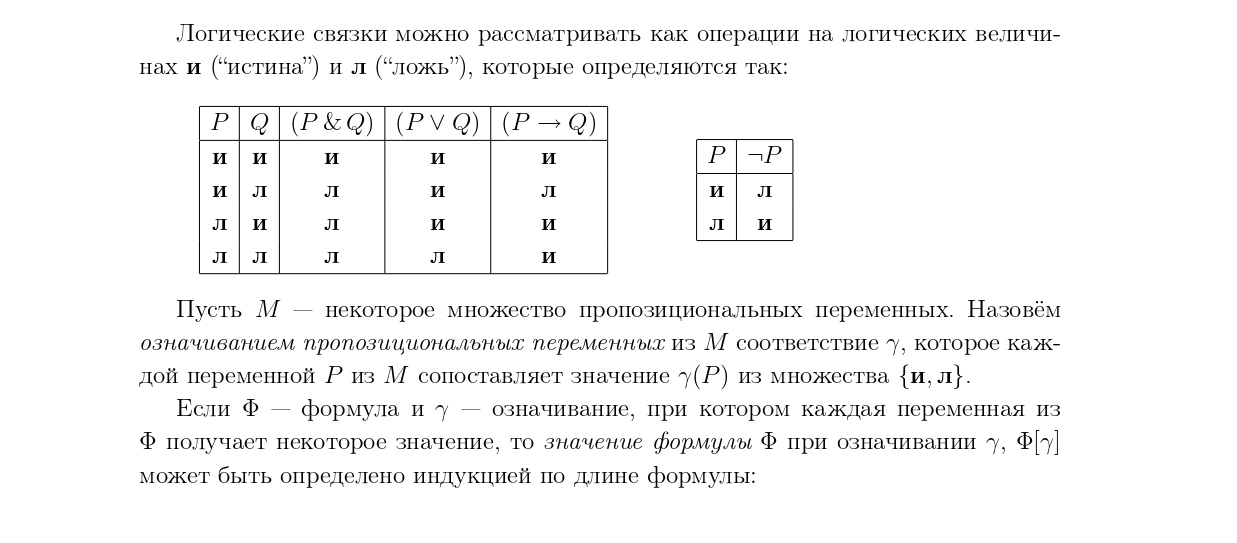
\includegraphics[scale=0.4]{32_1.jpg}\\
       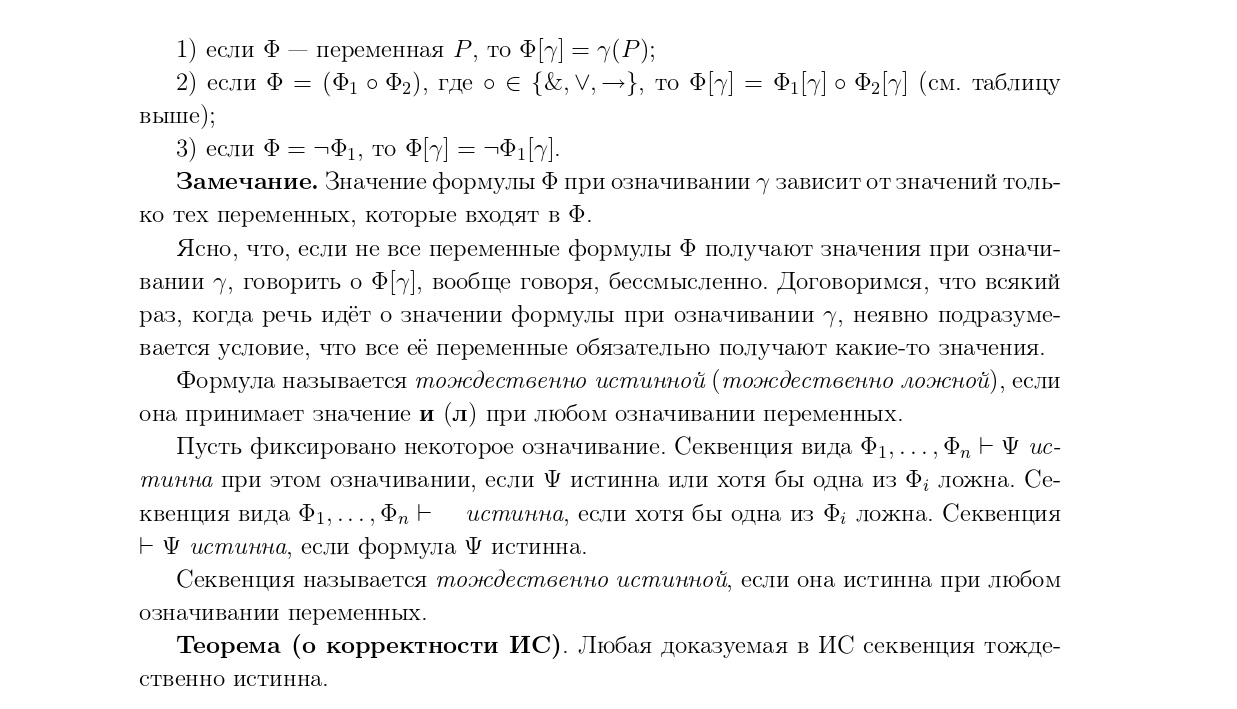
\includegraphics[scale=0.4]{32_2.jpg}\\
       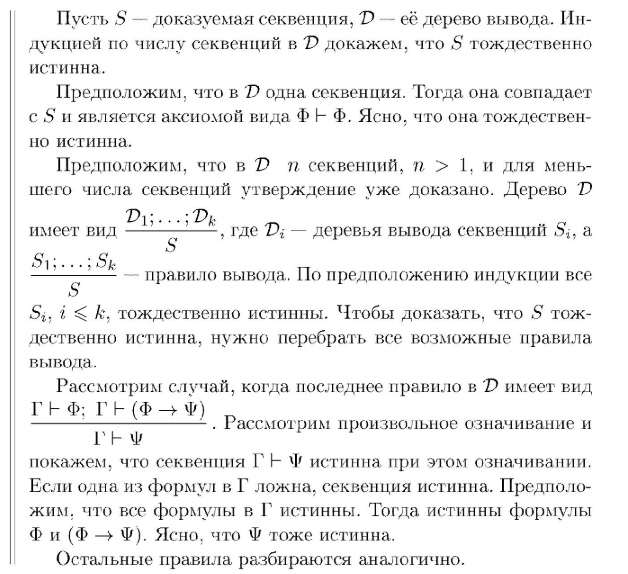
\includegraphics[scale=0.7]{32_3.jpg}
 \item Тождественно истинные секвенции, теорема о корректности ИС.
       \begin{definition*}[Тождественно истинные секвенции]
        Секвенция называется тождественно истинной, если она истинна при любом означивании входящих в неё переменных.
       \end{definition*}
       \begin{theorem*}[о корректности ИС]
        Любая доказуемая в ИС секвенция тождественно истинна.
       \end{theorem*}
       \begin{proof}
        Пусть $S$ - доказуемая секвенция, $D$ - её дерево вывода. Индукцией по числу секвенций в $D$ докажем, что $S$ тождественно истинна.\\
        Предположим, что в $D$ одна секвенция. Тогда она совпадает с $S$ и является аксиомой вида $\Phi \vdash \Phi$. Ясно, что она тождественно истинна.\\
        Предположим, что в $D$ $n$ секвенций, $n > 1$, и для меньшего числа секвенций утверждение уже доказано. Дерево $D$ имеет вид $\frac{D_1;...;D_k}{S}$, где $D_i$ - деревья вывода секвенций $S_i$, а $\frac{S_1;...; S_k}{S}$ - правило вывода. По предположению индукции все $S_i$, $i \leq k$, тождественно истинны. Чтобы доказать, что $S$ тождественно истинна, нужно перебрать все возможные правила вывода.\\
        Рассмотрим случай, когда последнее правило в $D$ имеет вид $\frac{\Gamma \vdash \Phi; \Gamma \vdash (\Phi \rightarrow \Psi)}{\Gamma \vdash \Psi}$. Рассмотрим произвольное означивание и покажем, что секвенция $\Gamma \vdash \Psi$ истинна при этом означивании. Если одна из формул в $\Gamma$ ложна, секвенция истинна. Предположим, все формулы в $\Gamma$ истинны. Тогда истинны формулы $\Phi$ и $(\Phi \rightarrow \Psi)$. Ясно, что $\Psi$ тоже истинна.\\
        Остальные правила разбираются аналогично.
       \end{proof}
 \item Допустимые правила вывода, примеры.
       \mbox{}\\ 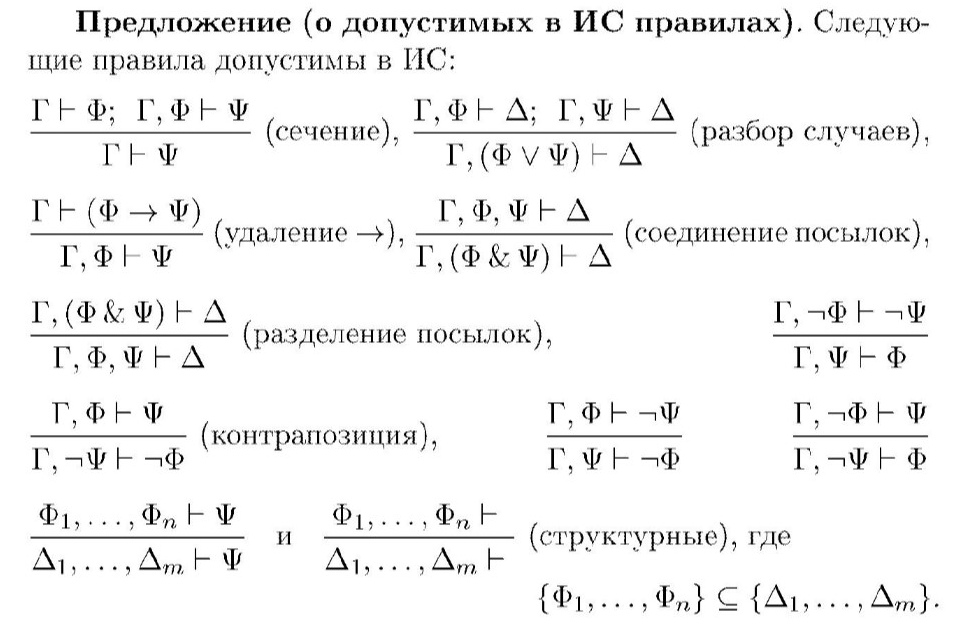
\includegraphics[scale=0.4]{34_1.jpg}\\
       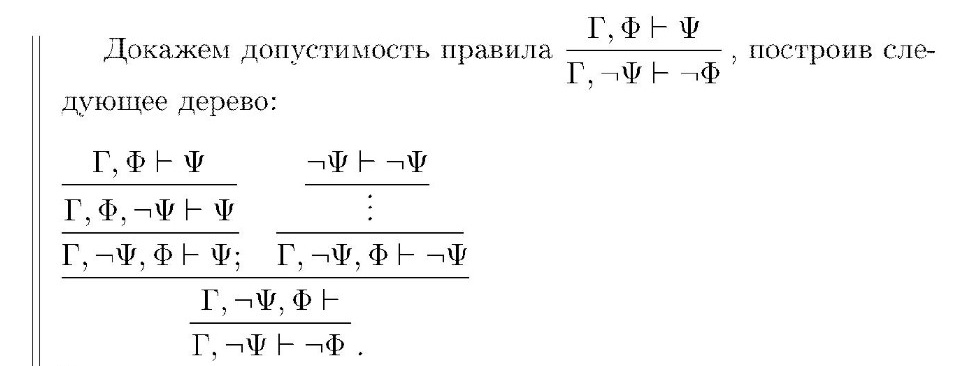
\includegraphics[scale=0.4]{34_2.jpg}\\
       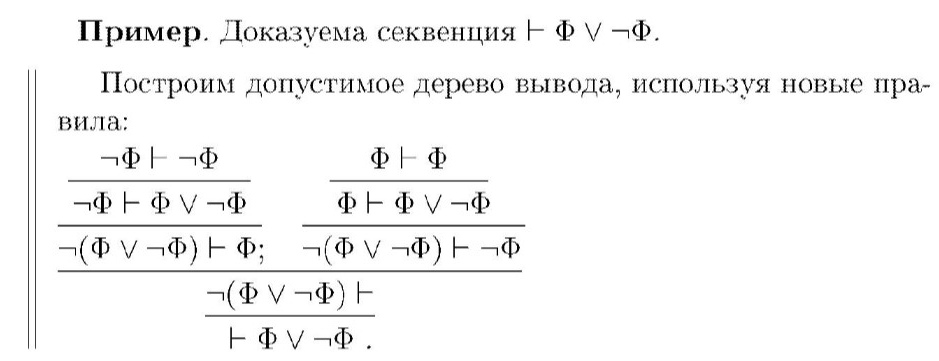
\includegraphics[scale=0.4]{34_3.jpg}
 \item Лемма об основных эквивалентностях, теорема о замене для ИВ.
       \begin{lemma*}[об основных эквивалентностях]
        Для любых формул $\Phi, \Psi, \Phi^{'}, \Psi^{'} \text{ и } \Delta$ верно:
        \begin{enumerate}
         \item $\Phi \equiv \Phi$;
         \item $\Phi \equiv \Psi \Rightarrow \Psi \equiv \Phi$;
         \item $\Phi \equiv \Psi, \Psi \equiv \Delta \Rightarrow \Phi \equiv \Delta$;
         \item $\Phi \equiv \Phi^{'}\Rightarrow \lnot \Phi \equiv \lnot \Phi^{'}$;
         \item $\Phi \equiv \Phi^{'}, \Psi \equiv \Psi^{'} \Rightarrow (\Phi^{'} \circ \Psi) \equiv (\Phi^{'} \circ \Psi^{'})$, где $\circ \in \{\ \&, \vee, \rightarrow\}$.
        \end{enumerate}
       \end{lemma*}
       \begin{proof}
        Пункты $a), b)$ очевидны; с): предположим, что доказуемы секвенции $\Phi \vdash \Psi, \Psi \vdash \Phi, \Psi \vdash \Delta, \Delta \vdash \Psi$. Покажем доказуемость секвенции $\Phi \vdash \Delta$, построив допустимое дерево:\\
        \begin{displaymath}
         \prftree
         {\prfassumption{\Phi \vdash \Psi}} {\prftree{\prfassumption{\Phi \vdash \Delta}}{\Phi, \Psi \vdash \Delta}}
         {\Phi \vdash \Delta}
        \end{displaymath}
        Дерево для $\Delta \vdash \Phi$ строится симметрично. Далее будем указывать только деревья.\\
        $d):$
        \begin{displaymath}
         \prftree
         {\Phi^{'} \vdash \Phi}
         {\neg \Phi \vdash \neg \Phi^{'}}
        \end{displaymath}
        $e):$ построим три дерева для случаев $\circ = \rightarrow, \circ = \&$ и $\circ = \vee$. Далее мы иногда будем пропускать структурные правила, соединяя несколько структурных правил с одним основным или допустимым в один переход дерева.
        \begin{displaymath}
         \prftree
         {\prftree
          {\prftree
           {\Phi^{'} \vdash \Phi;}{(\Phi \rightarrow \Psi) \vdash (\Phi \rightarrow \Psi)}
           {(\Phi \rightarrow \Psi), \Phi^{'} \vdash \Psi;}} {\prftree{\Psi \vdash \Psi^{'}}{(\Phi \rightarrow \Psi), \Phi^{'}, \Psi \vdash \Psi^{'}}}
          {{(\Phi \rightarrow \Psi), \Phi^{'} \vdash \Psi^{'}}}
         }
         {(\Phi \rightarrow \Psi) \vdash (\Phi^{'} \rightarrow \Psi{'})}
        \end{displaymath}
        \begin{multicols}{2}
         \begin{displaymath}
          \prftree
          {\prftree
           {\prftree
            {\Phi \vdash \Phi^{'}}
            {\Phi, \Psi \vdash \Phi^{'}}}
           {(\Phi \& \Psi) \vdash \Phi^{'};}}{\prftree
           {\prftree
            {\Psi \vdash \Psi^{'}}
            {\Phi, \Psi \vdash \Psi^{'}}}
           {(\Phi \& \Psi) \vdash \Psi{'}}}
          {(\Phi \& \Psi) \vdash (\Phi^{'} \& \Psi^{'})}
         \end{displaymath}
         \columnbreak
         \\ \\
         \begin{displaymath}
          \prftree
          {\prftree
           {\Phi \vdash \Phi^{'}}
           {\Phi \vdash (\Phi^{'} \vee \Psi^{'});}}{
           \prftree
           {\Psi \vdash \Psi^{'}}
           {\Psi \vdash (\Phi^{'} \vee \Psi^{'})}}
          {(\Phi \vee \Psi) \vdash (\Phi^{'} \vee \Psi^{'})}
         \end{displaymath}
        \end{multicols}
       \end{proof}
       \begin{theorem*}[о замене для ИВ]
        Пусть $\Psi$ - подформула формулы $\Phi$. Обозначим через $\Phi^{'}$ результат замены $\Psi$ на $\Psi^{'}$. Если $\Psi \equiv \Psi^{'}$, то и $\Phi \equiv \Phi^{'}$.
       \end{theorem*}
       \begin{proof}
        Индукцией по $|\Phi|$ докажем, что $\Phi^{'}$ - формула, эквивалентная $\Phi$. Если $\Phi = \Psi$, то $\Phi^{'} = \Psi^{'}$ и $\Phi \equiv \Phi^{'}$. Поэтому будем рассматривать только случай $\Phi \neq \Psi$.\\
        Пусть $|\Phi| = 1$. Тогда $\Phi = \Psi$, и этот случай уже рассмотрен.\\
        Пусть $|\Phi| > 1$, и для формул меньшей длины утверждение уже доказано. Если $\Phi =  \neg \Phi_1$, то $\Psi$ - подформула $\Phi_1$, и по предположению индукции $\Phi_1 \equiv \Phi^{'}_1$. Тогда $\Phi = \neg \Phi_1 \equiv \neg \Phi^{'}_1 = \Phi^{'}$ \\
        Если $\Phi = (\Phi_1 \circ \Phi_2)$, где $\circ \in \{\&, \vee, \rightarrow\}$, то $\Psi$ - подформула $\Phi_1$ или $\Phi_2$. Предположим, что $\Psi$ - подформула $\Phi_1$. По предположению индукции $\Phi_1 \equiv \Phi^{'}_1$, отсюда $\Phi = (\Phi_1 \circ \Phi_2) \equiv (\Phi^{'}_1 \circ \Phi_2) = \Phi^{'}$.
       \end{proof}
 \item Д.н.ф., к.н.ф., теорема о приведении к д.н.ф. и к.н.ф.
       \mbox{}\\ 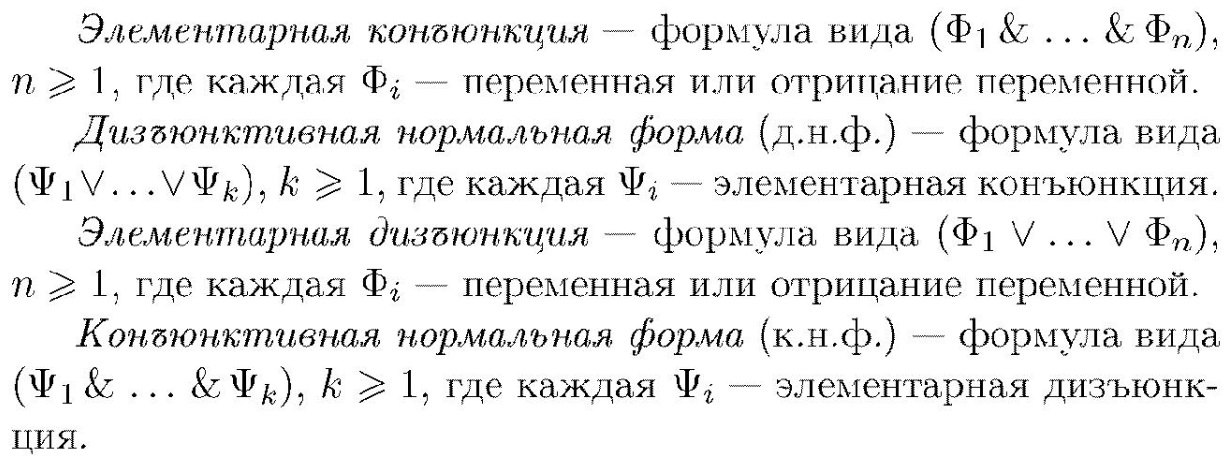
\includegraphics[scale=0.45]{36_1.jpg}\\
       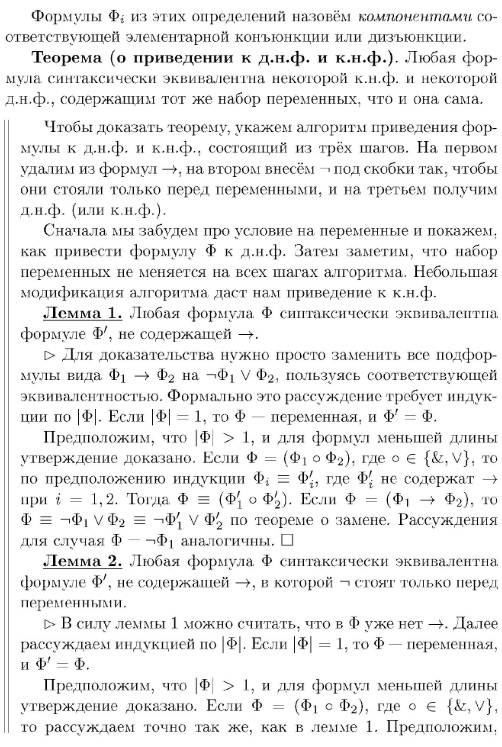
\includegraphics[scale=0.93]{36_2.jpg}\\
       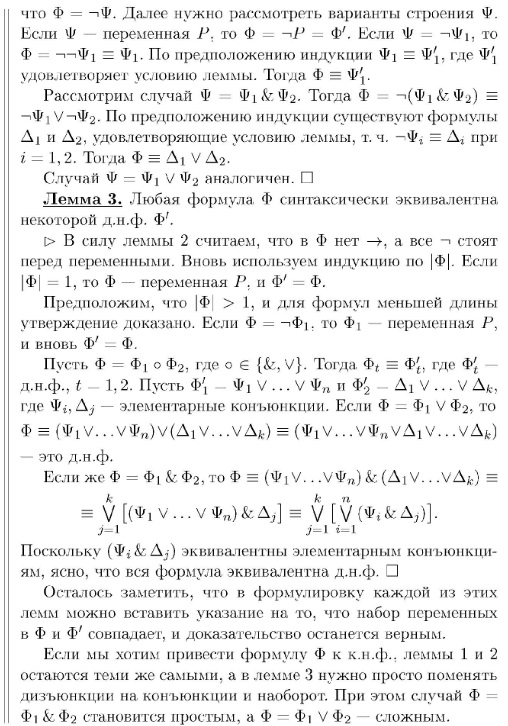
\includegraphics[scale=0.93]{36_3.jpg}
 \item Предложение о тождественно истинных к.н.ф.
       \mbox{}\\ 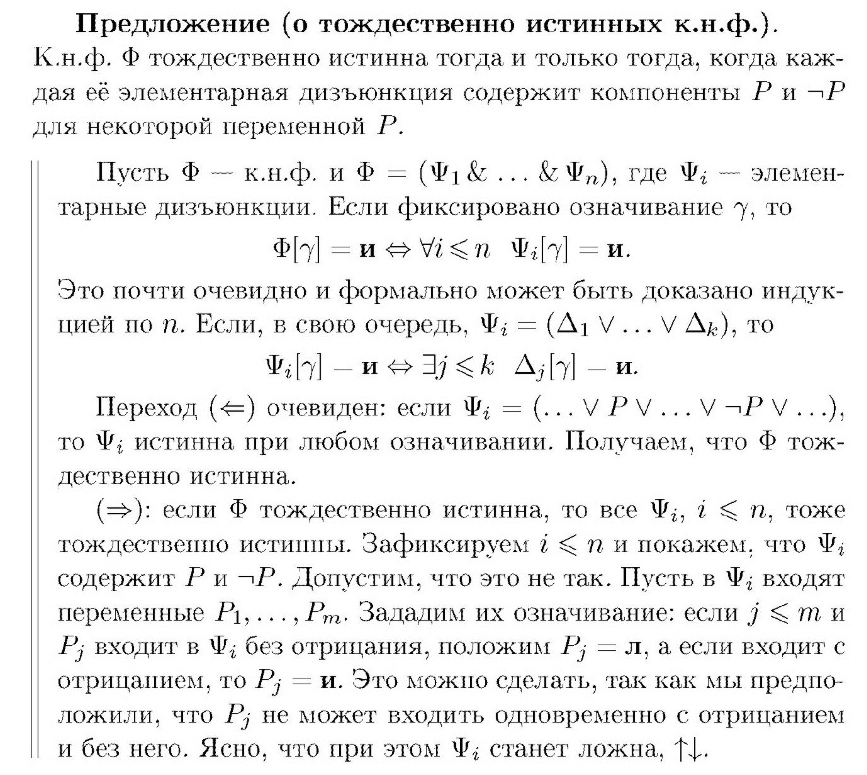
\includegraphics[scale=0.45]{37.jpg}
 \item Теорема о полноте ИС.
       \mbox{}\\ 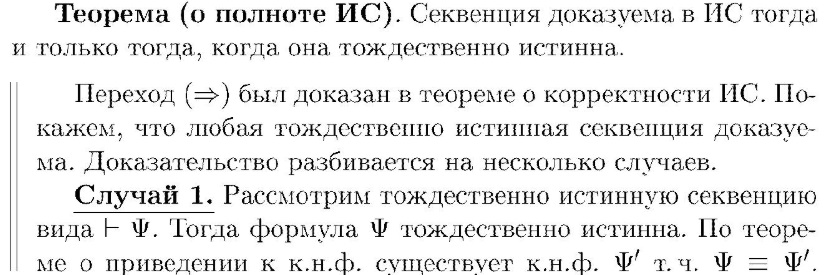
\includegraphics[scale=0.6]{38_1.jpg}\\
       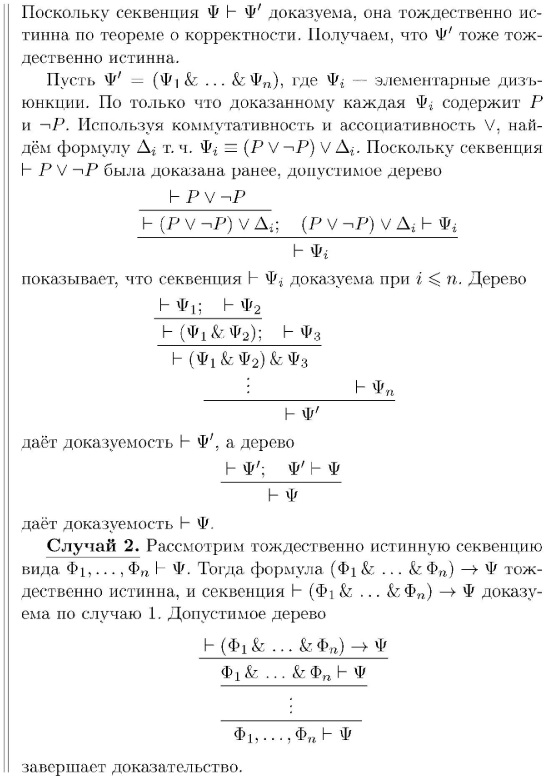
\includegraphics[scale=0.89]{38_2.jpg}\\
       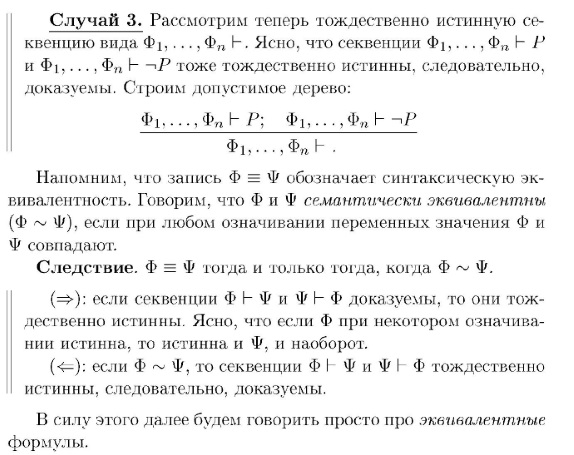
\includegraphics[scale=0.89]{38_3.jpg}
 \item Совершенные нормальные формы, теорема о совершенных нормальных формах.
       \mbox{}\\ 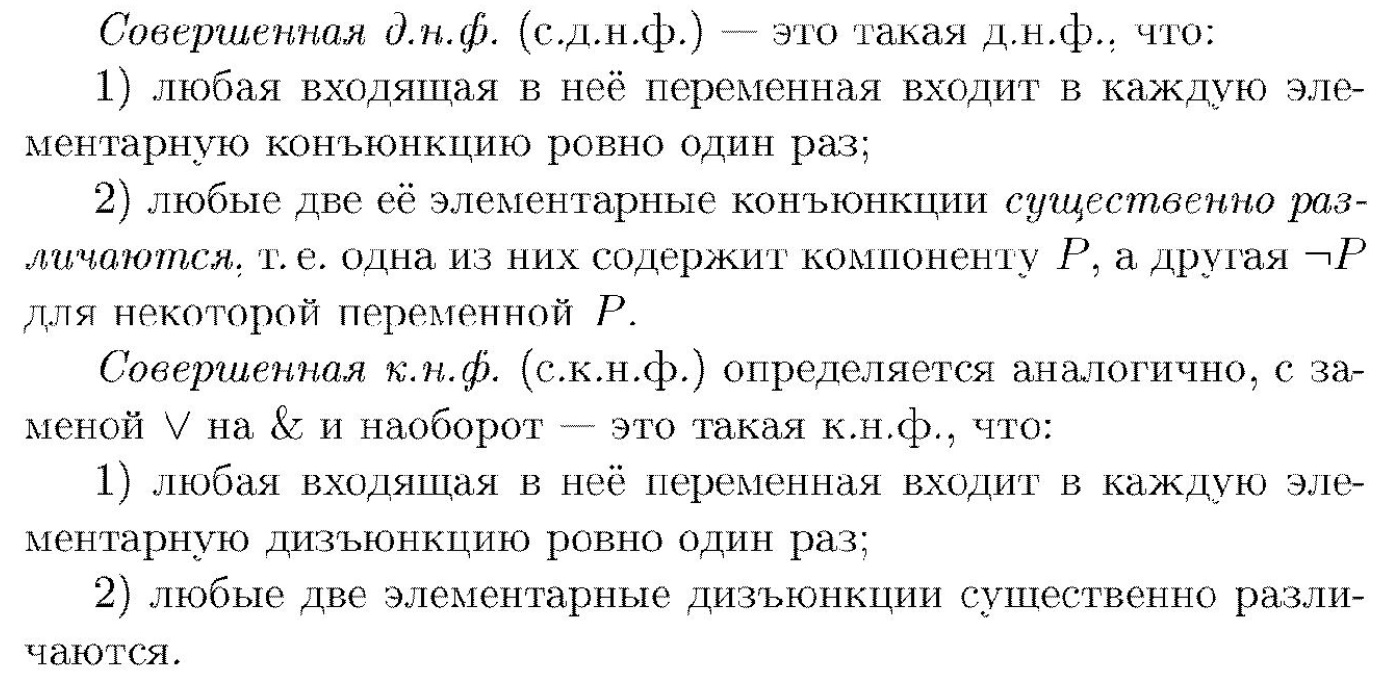
\includegraphics[scale=0.4]{39_1.jpg}\\
       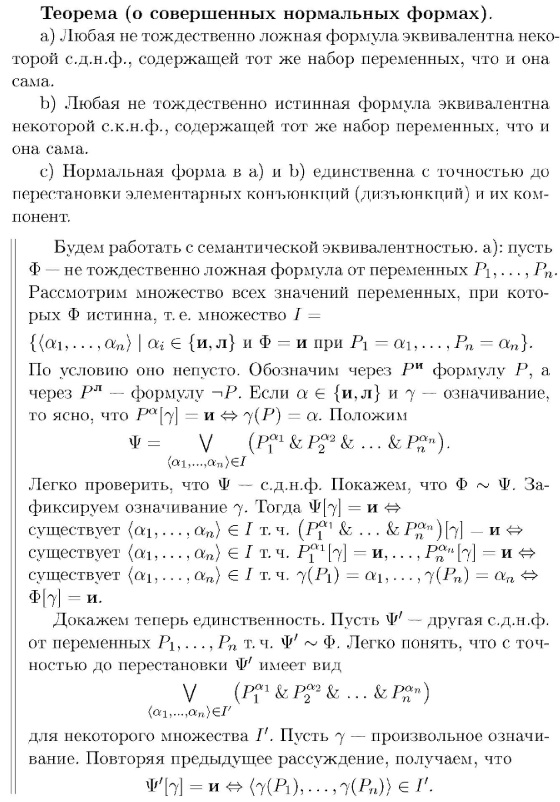
\includegraphics[scale=0.9]{39_2.jpg}\\
       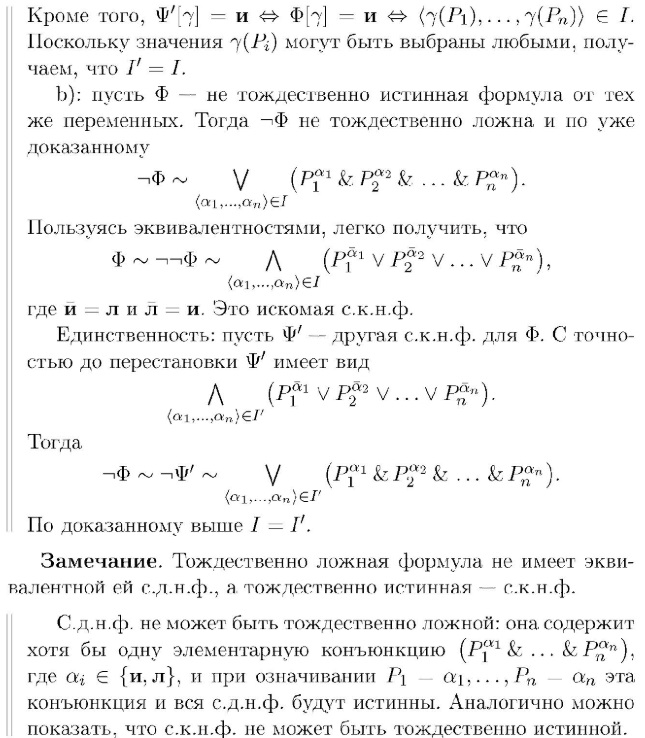
\includegraphics[scale=0.75]{39_3.jpg}
 \item Гильбертовское исчисление высказываний: аксиоматика, выводимость, примеры выводов.\\
       \textbf{Гильбертовское исчисление высказываний}\\
       \textbf{Аксиоматика}:\\
       1) $(\phi \to (\psi \to \phi))$\\
       2) $((\phi \to \psi)\to((\phi \to (\psi \to \chi))\to (\phi\to\chi) ))$\\
       3) $((\phi\ \&\ \psi)\to\phi)$\\
       4) $((\phi\ \&\ \psi)\to\psi)$\\
       5.1) $(\phi \to (\psi \to (\phi\ \&\ \psi)))$\\
       5.2) $((\phi \to \psi)\to((\phi \to \chi)\to(\phi\to(\psi\ \&\ \chi))))$\\
       6) $(\phi \to (\phi \lor \psi))$\\
       7) $(\psi \to (\phi \lor \psi))$\\
       8) $((\phi \to \psi)\to((\chi \to \psi)\to((\phi \lor \chi)\to\psi)))$\\
       9.1) $((\phi \to \lnot \psi)\to(\psi \to \lnot \phi))$\\
       9.2) $((\phi \to \psi)\to((\phi\to\lnot\psi)\to\lnot\phi))$\\
       10)  $\lnot\lnot\phi\to\phi$\\
       \textbf{Правило modes ponens}:
       $\frac{\phi, (\phi \to \psi)}{\psi}$
       \begin{definition*}[Вывод формулы в ГИВ]
        Выводом формулы $\phi$ в ГИВ называется последовательностью формул, каждой из которых является либо аксиомой, либо полученна из предыдущего по правилу modes ponens. \\
        Последнее из вывода есть вывод $\phi$
       \end{definition*}
       \begin{theorem*}
        Выводом $\phi$ из $\Gamma$, называется последовательность формул, каждая из которых либо является аксиомой, либо принадлежащая $\Gamma$, либо следует из двух предыдущих по правилу modes ponens.\\
        Последняя формула в последовательности это $\phi$
       \end{theorem*}
 \item Теорема о дедукции.
       \begin{theorem*}[о дедукции]
        Если $\Gamma, A \triangleright B$, то $\Gamma \triangleright A\to{B}$
       \end{theorem*}
       \begin{proof}
        Пусть $B_1,..., B_n = B$ - вывод $B$ из $\Gamma, A$\\
        По индукции докажем, что $\forall{i} \Gamma\triangleright{A\to{B}}$
        \begin{itemize}
         \item $B_i\in \Gamma$:\\
               1) $B_i \in \Gamma$
               2) $(B_i \to (A\to{B_i}))$ - Аксиома №1
               3) $A \to B_i$ - mp 1,2
         \item $B_i$ - следствие из $B_j$ и $B_j\to{B_i}$ по mp:
               \\ По Индукционной гипотезе :
               $\Gamma \triangleright (A\to{B_j})$,
               $\Gamma \triangleright (A\to{(B_j \to {B_i})})$\\
               .\\.\\.\\
               n) $(A \to B_j)$\\
               .\\.\\.\\
               m) $(A \to (B_j \to B_i))$\\
               m+1) $((A \to B_j)\to((A\to(B_j\to{B_i}))\to(A\to{B_i})))$ - Аксиома №2\\
               m+2) $(((A\to(B_j\to{B_i}))\to(A\to{B_i}))$ - mp n,m+1\\
               m+3) $(A\to{B_i})$ - mp m, m+2
        \end{itemize}
       \end{proof}
 \item Связь гильбертовского и секвенциального исчисления.
       ?????
\end{enumerate}
\end{document}
